% \documentclass[sigplan,10pt]{acmart}\settopmatter{printfolios=true}
\documentclass[acmsmall,10pt]{acmart}\settopmatter{printfolios=true}
%% For final camera-ready submission
%\documentclass[sigplan,10pt]{acmart}\settopmatter{}

\settopmatter{printacmref=false} % Removes citation information below abstract
\renewcommand\footnotetextcopyrightpermission[1]{} % removes footnote with conference information in first column
\pagestyle{plain} % removes running headers

%% Some recommended packages.
\usepackage{booktabs}   %% For formal tables:
                        %% http://ctan.org/pkg/booktabs
\usepackage{subcaption} %% For complex figures with subfigures/subcaptions
                        %% http://ctan.org/pkg/subcaption

\usepackage{array}
\usepackage[section]{placeins}
\usepackage{mathpartir}
\usepackage{xcolor}
\usepackage{xspace}
\usepackage{stmaryrd}
\usepackage{listings}
\usepackage{newtxmath}
\usepackage{framed}

%% Tikz Needed packages
\usepackage{pgfplots}
\pgfplotsset{width=7cm,compat=1.8}
\usepackage{pgfplotstable}
\renewcommand*{\familydefault}{\sfdefault}

%\makeatletter\if@ACM@journal\makeatother
%%% Journal information (used by PACMPL format)
%%% Supplied to authors by publisher for camera-ready submission
%\acmJournal{ICFP 17 student research competition}
%\acmVolume{1}
%\acmNumber{1}
%\acmArticle{1}
%\acmYear{2017}
%\acmMonth{1}
%\acmDOI{10.1145/nnnnnnn.nnnnnnn}
%\startPage{1}
%\else\makeatother
%%% Conference information (used by SIGPLAN proceedings format)
%%% Supplied to authors by publisher for camera-ready submission
%\acmConference[ICFP 2017 Student Research Competition]{ICFP 2017 Student Research Competition}{September, 2017}{Oxford, UK}
%\acmYear{2017}
%\acmISBN{978-x-xxxx-xxxx-x/YY/MM}
%\acmDOI{10.1145/nnnnnnn.nnnnnnn}
%\startPage{1}
%\fi

%% Copyright information
%% Supplied to authors (based on authors' rights management selection;
%% see authors.acm.org) by publisher for camera-ready submission
\setcopyright{none}             %% For review submission
%\setcopyright{acmcopyright}
%\setcopyright{acmlicensed}
%\setcopyright{rightsretained}
%\copyrightyear{2017}           %% If different from \acmYear

%% Bibliography style
\bibliographystyle{ACM-Reference-Format}
%% Citation style
%% Note: author/year citations are required for papers published as an
%% issue of PACMPL.
%\citestyle{acmauthoryear}  %% For author/year citations
%\citestyle{acmnumeric}     %% For numeric citations
%\setcitestyle{nosort}      %% With 'acmnumeric', to disable automatic
                            %% sorting of references within a single citation;
                            %% e.g., \cite{Smith99,Carpenter05,Baker12}
                            %% rendered as [14,5,2] rather than [2,5,14].
%\setcitesyle{nocompress}   %% With 'acmnumeric', to disable automatic
                            %% compression of sequential references within a
                            %% single citation;
                            %% e.g., \cite{Baker12,Baker14,Baker16}
                            %% rendered as [2,3,4] rather than [2-4].

\newcommand{\lang}{\textsc{Effy}\xspace}
\newcommand{\eff}{\textsc{Eff}\xspace}
\newcommand{\core}{\textsc{EffCore}\xspace}
\newcommand{\ocaml}{\textsc{OCaml}\xspace}

% Meta-syntax
\newcommand{\bnfis}{\mathrel{\;{:}{:}\!=}\;}
\newcommand{\bnfor}{\mathrel{\;|\;}}
\newcommand{\defeq}{\mathrel{\;\stackrel{\text{def}}{=}\;}}
\newcommand{\set}[1]{\{ #1 \}}

% General syntactic constructs
\newcommand{\kord}[1]{\mathtt{#1}}
\newcommand{\kop}[1]{\;\mathtt{#1}\;}
\newcommand{\kpre}[1]{\mathtt{#1}\;}
\newcommand{\kpost}[1]{\;\mathtt{#1}}

% Types
\newcommand{\type}[1]{\mathtt{#1}}
\newcommand{\boolty}{\type{bool}}
\newcommand{\intty}{\type{int}}
\newcommand{\hto}{\Rightarrow}
\renewcommand{\C}{\underline{C}}
\newcommand{\D}{\underline{D}}
\newcommand{\dirt}{\Delta}
\newcommand{\dirtend}{. (\textsc{dot})}
\newcommand{\sig}{\Sigma}
\newcommand{\allops}{\Omega}

% Expressions and computations
\newcommand{\funtyped}[3]{\kpre{fun} #1 \T #2 \mapsto #3}
\newcommand{\rectype}[1]{\mu \alpha . #1}
\newcommand{\letvar}{\textbf{\^{x}}}
\newcommand{\union}{\sqcup}
\newcommand{\intersection}{\sqcap}
\newcommand{\emptyrow}{\emptyset}
\newcommand{\polytype}[1]{\forall \bar{\alpha} . #1}

\newcommand{\call}[3]{{{#1}\,{#2}\,{#3}}}
\newcommand{\case}{\mathop{\text{\texttt{|}}}}
\newcommand{\cont}[2]{(#1.\,#2)}
\newcommand{\const}{\kord{k}}
\newcommand{\fls}{\kord{false}}
\newcommand{\fun}[1]{\lambda #1 .} %\kpre{fun} #1 \mapsto}
\newcommand{\handler}[1]{\{ #1 \}}
\newcommand{\conditional}[3]{\kpre{if} #1 \kop{then} #2 \kop{else} #3}
\newcommand{\letin}[1]{\kpre{let} #1 \kop{in}}
\newcommand{\doin}[1]{\kpre{do} #1 \kop{ ; }}
\newcommand{\letrecin}[1]{\kpre{let} \kpre{rec} #1 \kop{in}}
\newcommand{\op}{\kord{Op}}
\newcommand{\ops}{\mathcal{O}}
\newcommand{\ocs}{\mathit{ocs}}
\newcommand{\ocsnil}{\kord{nil}}
\newcommand{\tru}{\kord{true}}
\newcommand{\ret}{\kpre{return}}
\newcommand{\withhandle}[2]{\kpre{handle} #2 \kop{with} #1}
\newcommand{\pure}[1]{\kord{pure } #1  }
\newcommand{\longcases}{\call{\op_1}{y}{k} \mapsto c_{\op_1}, \ldots, \call{\op_n}{x}{k} \mapsto c_{\op_n}}
\newcommand{\shortcases}{[\call{\op}{y}{k} \mapsto c_\op]_{\op \in \ops}}
\newcommand{\longhand}[1][\ret x \mapsto c_r]{\handler{#1, \longcases}}
\newcommand{\shorthand}[1][\ret x \mapsto c_r]{\handler{#1, \shortcases}}
\newcommand{\shorthandelab}[1][\ret x \mapsto c'_r]{\handler{#1, \shortcaseselab}}
\newcommand{\shortcaseselab}{[\call{\op}{y}{k} \mapsto c'_\op]_{\op \in \ops}}

% Type-checking
\newcommand{\row}{\mathrel{;} R}
\newcommand{\ctx}{\Gamma}
\newcommand{\ctxm}{\Xi}
\newcommand{\ctxp}{\Pi}
\newcommand{\ent}{\vdash}
\newcommand{\entt}{\Vdash}
\newcommand{\T}{\mathrel{:}}
\newcommand{\E}{\mathrel{!}}
\newcommand{\covers}{\mathrel{/}}
\renewcommand{\le}{\leqslant}

% Operational semantics
\newcommand{\eval}{\Downarrow}
\newcommand{\hs}{\mathcal{H}}
\newcommand{\nil}{\emptyset}
\newcommand{\cons}{\mathbin{::}}
\newcommand{\hseval}[1][\hs]{\Downarrow_{#1}}
\newcommand{\getval}[1]{{#1}_{\kord{val}}}
\newcommand{\getop}[1]{{#1}_{\kord{op}}}

\newcommand{\todo}[1]{\textcolor{red}{\textsc{Todo:} #1}}

\begin{document}

\title{Algebraic subtyping for algebraic effects and handlers}

\author{Axel Faes}
\affiliation{
  \position{student : undergraduate\\ACM Student Member: 2461936}
  \department{Department of Computer Science}
  \institution{KU Leuven}
}
\email{axel.faes@student.kuleuven.be}

\author{Amr Hany Saleh}
\affiliation{
  \position{daily advisor}
  \department{Department of Computer Science}
  \institution{KU Leuven}
}
\email{amrhanyshehata.saleh@kuleuven.be }

\author{Tom Schrijvers}
\affiliation{
  \position{promotor}
  \department{Department of Computer Science}
  \institution{KU Leuven}
}
\email{tom.schrijvers@kuleuven.be}

%% Keywords
%% comma separated list
\keywords{algebraic effect handler, algebraic subtyping, effects, optimised compilation}  %% \keywords is optional

%% Abstract
%% Note: \begin{abstract}...\end{abstract} environment must come
%% before \maketitle command
\begin{abstract}
  Algebraic effects and handlers benefit from a custom type-\&-effect system, a type system that also tracks which effects can happen in a program. Several such type-\&-effect systems have been proposed in the literature, but all are unsatisfactory. Recently, Stephen Dolan (University of Cambridge, UK) presented a novel type system that combines subtyping and parametric polymorphism in a particulary attractive and elegant fashion. A cornerstone of his design are the algebraic properties that the subtyping relation should respect. In this work, a type-\&-effect system is derived that extends Dolan's elegant type system with effect information. This type-\&-effect system inherits Dolan's harmonious combination of subtyping (in our case induced by a lattice structure on the effect information) with parametric polymorphism and preserves all of its desirable properties (both low-level algebraic properties and high-level meta-theoretical properties like type soundness and the existence of principal types).
\end{abstract}

\maketitle

\tableofcontents

\listoffigures
\listoftables

% \chapter{Introduction}
% The specification for a type-\&-effect system with algebraic subtyping for algebraic effects and handlers is given in this document. The formal properties of this system are studied in order to find which properties are satisfied compared to other type-\&-effect systems. The proposed type-\&-effect system builds on two very recent developments in the area of programming language theory.

\paragraph{Algebraic subtyping}
In his December 2016 PhD thesis, Stephen Dolan (University of Cambridge, UK), has presented a novel type system that combines subtyping and parametric polymorphism in a particulary attractive and elegant fashion. A cornerstone of his design are the algebraic properties that the subtyping relation should respect.

\paragraph{Algebraic effects and handlers}
These are a new formalism for formally modelling side-effects (e.g. mutable state or non-determinism) in programming languages, developed by Matija Pretnar (University of Ljubjana) and Gordon Plotkin (University of Edinburgh). This approach is gaining a lot of traction, not only as a formalism but also as a practical feature in actual programming languages (e.g. the Koka language developed by Microsoft Research). We are collaborating with Matija Pretnar on the efficient implementation of one such language, called Eff. Axel Faes has contributed to this collaboration during a project he did for the Honoursprogramme of the Faculty of Engineering Science.

\subsection{Motivation}
Algebraic effects and handlers benefit from a custom type-\&-effect system, a type system that also tracks which effects can happen in a program. Several such type-\&-effect systems have been proposed in the literature, but all are unsatisfactory. We attribute this to the lack of the elegant properties of Dolan's type system. Indeed the existing type-\&-effect systems are not only theoretically unsatisfactory, but they are also awkward to implement and use in practice.

\paragraph{Research questions}
\begin{itemize}
\item How can Dolan's elegant type system be extended with effect information?
\item Which properties are preserved and which aren't preserved?
\item What advantages are there to an type-\&-effect system based on Dolan's elegant type system?
\end{itemize}

\subsection{Goals}
The goal of this thesis is to derive a type-\&-effect system that extends Dolan's elegant type system with effect information. This type-\&-effect system should inherit Dolan's harmonious combination of subtyping (in our case induced by a lattice structure on the effect information) with parametric polymorphism and preserve all of its desirable properties (both low-level algebraic properties and high-level meta-theoretical properties like type soundness and the existence of principal types). Afterwards this type-\&-effect system The following approach is taken:
\begin{enumerate}
\item Study of the relevant literature and theoretical background.
\item Design of a type-\&-effect system derived from Dolan's, that integrates effects.
\item Proving the desirable properties of the proposed type-\&-effect system: type soundness, principal typing, ...
\item Time permitting: Design of a type inference algorithm that derives the principal types of programs without type annotations and proving its correctness.
\item Time permitting: Implementation of the algorithm and comparing it to other algorithms (such as row polymorphism based type-\&-effect systems).
\end{enumerate}

\subsection{Results}
Describe what the resulting product is and how it is useful or provides an advantage over other solutions.

% \chapter{Background}
% \section{Simply Typed Lambda Calculus}
% In this section, I will provide the background necessary to be able to read the text. This includes an introduction into programming languages (and programming language theory) and algebraic effect handlers 

Dolan's type system and \eff are discussed in further chapters and thus shouldn't need to be explained in this section.

% \section{Algebraic effects and handlers (\eff)}
% The type-\&-effect system that is used in \eff is based on subtyping and dirty types \cite{effectsystem}.

% \subsection{Types and terms}

\paragraph{Terms}
Figure~\ref{fig:terms:eff} shows the two types of terms in \eff. There are values $v$ and computations $c$. Computations are terms that can contain effects. Effects are denoted as operations $Op$ which can be called.

\begin{figure}[!htb]
\begin{center}
\framebox{
\begin{minipage}{0.98\columnwidth}
\[\begin{array}{r@{~}c@{~}l@{\quad}l}
  \text{value}~v & \bnfis {} & x & \text{variable} \\ %\lambda\text{-variable} \\
    % & \bnfor & \letvar & \text{let-variable} \\
    % & \bnfor & \const & \text{constant} \\
    & \bnfor & \tru & \text{true} \\
    & \bnfor & \fls & \text{false} \\
    & \bnfor & \fun{x} c & \text{function} \\
    & \bnfor & \{ & \text{handler} \\
    & & \quad \ret x \mapsto c_r, & \quad\text{return case} \\
    & & \quad \shortcases & \quad\text{operation cases} \\
    & & \} & \\
  \text{comp}~c & \bnfis & v_1 \, v_2 & \text{application} \\
    & \bnfor & \doin{x \leftarrow c_1} c_2 & \text{sequencing} \\
    & \bnfor & \conditional{e}{c_1}{c_2} & \text{conditional} \\
    & \bnfor & \letrecin{f \, x = c_1} c_2 & \text{rec definition} \\
    & \bnfor & \ret v  & \text{returned val} \\
    & \bnfor & \op \, v & \text{operation call} \\
    & \bnfor & \withhandle{v}{c} & \text{handling}
\end{array}\]
\end{minipage}
}
\end{center}
\caption{Terms of \eff}\label{fig:terms:eff}
\end{figure}

\paragraph{Types}
Figure~\ref{fig:types:eff} shows the types of \eff. There are two main sorts of types. There are (pure) types $A, B$ and dirty types $\C, \D$. A dirty type is a pure type $A$ tagged with a finite set of operations $\dirt$, which we call dirt, that can be called. This finite set $\dirt$ is an over-approximation of the operations that are actually called. The type $\C \hto \D$ is used for handlers because a handler takes an input computation $\C$, handles the effects in this computation and outputs computation $\D$ as the result.

\begin{figure}[!htb]
\begin{center}
\framebox{
\begin{minipage}{0.98\columnwidth}
\[\begin{array}{r@{~}c@{~}l@{\quad}l}
  \text{(pure) type}~A, B & \bnfis {}
    % & \boolty \bnfor \intty & \text{basic types} \\
    & \boolty & \text{bool type} \\
    & \bnfor & A \to \C & \text{function type} \\
    & \bnfor & \C \hto \D & \text{handler type} \\
  \text{dirty type}~\C, \D & \bnfis {} & A \E \dirt \\
  \text{dirt}~\dirt & \bnfis {} &\set{\op_1, \dots, \op_n}
\end{array}\]
\end{minipage}
}
\end{center}
\caption{Types of \eff}\label{fig:types:eff}
\end{figure}

% \subsection{Subtyping}
The dirty type $A \E \dirt$ is assigned to a computation returning values of type $A$ and potentially calling operations from the set $\dirt$. This set $\dirt$ is always an over-approximation of the actually called operations, and may safely be increased, inducing a natural subtyping judgement $A \E \dirt \leq A \E \dirt'$ on dirty types. As dirty types can occur inside pure types, we also get a derived subtyping judgement on pure types. Both judgements are defined in Figure~\ref{fig:subtyping}. Observe that, as usual, subtyping is contravariant in the argument types of functions and handlers, and covariant in their return types. \cite{inferring}

\begin{figure}[!htb]
\begin{center}
\framebox{
\begin{minipage}{0.95\columnwidth}
\textbf{Subtyping}
\begin{mathpar}
  \inferrule[Sub-$\boolty$]{
  }{
    \boolty \le \boolty
  }

  \inferrule[Sub-$\to$]{
    A' \le A \\
    \C \le \C'
  }{
    A \to \C \le A' \to \C'
  }

  \inferrule[Sub-$\hto$]{
    \C' \le \C \\
    \D \le \D'
  }{
    \C \hto \D \le \C' \hto \D'
  }

  \inferrule[Sub-$\E$]{
    A \le A' \\
    \dirt \subseteq \dirt'
  }{
    A \E \dirt \le A' \E \dirt'
  }
\end{mathpar}
\end{minipage}
}
\end{center}
\caption{Subtyping for pure and dirty types of \eff}\label{fig:subtyping}
\end{figure}

\subsection{Typing rules}
Figure~\ref{fig:eff-typing} defines the typing judgements for values and computations with respect to a standard typing context $\ctx$.

\paragraph{Values}
The rules for subtyping, variables, and functions are entirely standard. For constants we assume a signature $\sig$ that assigns a type~$A$ to each constant~$\const$, which we write as $(\const \T A) \in \sig$.

A handler expression has type $A \E \dirt \cup \ops \hto B \E \dirt$ iff all branches (both the operation cases and the return case) have dirty type $B \E \dirt$ and the operation cases cover the set of operations $\ops$. Note that the intersection $\dirt \cap \ops$ is not necessarily empty. The handler deals with the operations $\ops$, but in the process may re-issue some of them (i.e., $\dirt \cap \ops$).

When typing operation cases, the given signature for the operation $(\op \T A_\op \to B_\op) \in \sig$ determines the type $A_\op$ of the parameter $x$ and the domain $B_\op$ of the continuation $k$. As our handlers are deep, the codomain of $k$ should be the same as the type $B \E \dirt$ of the cases. \cite{inferring}

\paragraph{Computations}
With the following exceptions, the typing judgement $\ctx \ent c : \C$ has a straightforward definition. The $\ret$ construct renders a value $v$ as a pure computation, i.e., with empty dirt. An operation invocation $\op\,v$ is typed according to the operation's signature, with the operation itself as its only operation. Finally, rule \textsc{With} shows that a handler with type $\C \hto \D$ transforms a computation with type $\C$ into a computation with type $\D$. \cite{inferring}

\begin{figure}[!htb]
\begin{center}
\framebox{
\begin{minipage}{0.95\columnwidth}
\[\begin{array}{r@{~}c@{~}l}
  \text{typing contexts}~\ctx & \bnfis {} & \epsilon \bnfor \ctx, x : A\\
\end{array}\]
\textbf{Expressions}
\begin{mathpar}
  \inferrule[SubVal]{
    \ctx \ent v \T A \\
    A \le A'
  }{
    \ctx \ent v \T A'
  }

  \inferrule[Var]{
    (x \T A) \in \ctx
  }{
    \ctx \ent x \T A
  }

  % \inferrule[Const]{
  %   (\const \T A) \in \sig
  % }{
  %   \ctx \ent \const \T A
  % }

  \inferrule[True]{
  }{
    \ctx \ent \tru \T bool
  }

  \inferrule[False]{
  }{
    \ctx \ent \fls \T bool
  }
  
  \inferrule[Fun]{
    \ctx, x \T A \ent c \T \C
  }{
    \ctx \ent \fun{x} c \T A \to \C
  }

  \inferrule[Hand]{
    \ctx, x \T A \ent c_r \T B \E \dirt \\
    \Big[
      (\op \T A_\op \to B_\op) \in \sig \qquad \\
      \ctx, y \T A_\op, k \T B_\op \to B \E \dirt \ent c_\op \T B \E \dirt
    \Big]_{\op \in \ops}
  }{
    \ctx \ent \shorthand \T \\ A \E \dirt \cup \ops \hto B \E \dirt
  }
\end{mathpar}
\textbf{Computations}
\begin{mathpar}
  \inferrule[SubComp]{
    \ctx \ent c \T \C \\
    \C \le \C'
  }{
    \ctx \ent c \T \C'
  }

  \inferrule[App]{
    \ctx \ent v_1 \T A \to \C \\
    \ctx \ent v_2 \T A
  }{
    \ctx \ent v_1 \, v_2 \T \C
  }

  \inferrule[Cond]{
    \ctx \ent v \T bool \\
    \ctx \ent c_1 \T \C \\
    \ctx \ent c_2 \T \C \\
  }{
    \ctx \ent \conditional{v}{c_1}{c_2} \T \C
  }

  \inferrule[LetRec]{
    \ctx, f \T A \to \C, x \T A \ent c_1 \T \C \\
    \ctx, f \T A \to \C \ent c_2 \T \D
  }{
    \ctx \ent \letrecin{f \, x = c_1} c_2 \T \D
  }

  \inferrule[Ret]{
    \ctx \ent v \T A
  }{
    \ctx \ent \ret v \T A \E \emptyset
  }

  \inferrule[Op]{
    (\op \T A \to B) \in \sig \\
    \ctx \ent v \T A
  }{
    \ctx \ent \op \, v \T B \E \{\op\}
  }

  \inferrule[Do]{
    \ctx \ent c_1 \T A \E \dirt \\
    \ctx, x \T A \ent c_2 \T B \E \dirt
  }{
    \ctx \ent \doin{x \leftarrow c_1} c_2 \T B \E \dirt
  }

  \inferrule[With]{
    \ctx \ent v \T \C \hto \D \\
    \ctx \ent c \T \C
  }{
    \ctx \ent \withhandle{v}{c} \T \D
  }
\end{mathpar}
\end{minipage}
}
\end{center}
\caption{Typing of \eff}\label{fig:eff-typing}
\end{figure}


% \section{Limitations}
% In the previous section, we discussed the background of algebraic effects and handlers as developed by Plotkin, Pretnar and Power \cite{DBLP:journals/acs/PlotkinP03, DBLP:conf/lics/PlotkinP08}. The system has been worked out and has been implemented as the Eff programming language of which the calculus has been described in the previous section. This was the first language to have effects as first class citizens \cite{pretnar2015introduction}. Algebraic effects and handlers aren't just a fancy new concept, it is quickly maturing. There is more and more adoption of algebraic effects as a practical language feature for user-defined side-effects. As language features are being adopted more and more, optimization becomes a bigger priority.

This section is a summerization of the work by Matija Pretnar et al. of which I was a co-author. This work focusses on the optimization of algebraic effect and handlers. First, we explain why optimizations of algebraic effects and handlers are needed. Afterwards, the optimizations are brievely discussed. Finally, some issues with the optimizations are given. The novelty of my thesis, while not being a solution to these issues, arises from the work done in the optimizations.

\subsection{Motivation}

Considering that multiple implementation are available, runtime performance becomes much more important. Some implementations take the form a interpreters \cite{programming, links2ocaml}. Most implementations take the form of libraries \cite{DBLP:conf/icfp/Brady13, kammar, eff2ocaml}. Most work has been towards the optimization of the runtime performance. However, in the case of Eff, there still was a performance difference of about 4400\% between the algebraic effects and hand-written code in OCaml (without algebraic effects). Another viable option was to provide an optimised compiler in order to transform the algebraic effects and handlers such that the runtime cost is avoided entirely \cite{optimization}. 

\subsection{Implementation}
There are two main ways that the optimising compiler used in order to optimise \eff code. The first is through the use of term rewriting rules, the other way is through purity aware compilation. Purity aware compilation provides a way for pure computations to have a more efficient representation, compared to the free monad representation. 

Several of the term rewriting rules that were created during the creation of the optimised compiler are given in figure~\ref{fig:rewriterules}. These rules show how terms are rewritten in order to minimize the footprint of algebraic effects and handlers.

\begin{figure}
\begin{center}
\framebox{
\begin{minipage}{0.95\columnwidth}
\textbf{Simplification}\\
\begin{mathpar}
  \inferrule[App-Fun]{
% \textit{inlinable}(x, e ,c)
  }{
    (\fun{x} c) \, v \leadsto c [v/x]
  }

%   \inferrule[Do-Ret]{
% % \textit{inlinable}(x, e ,c)
%   }{
%     \doin{x \leftarrow \ret v} c \leadsto c [v / x]
%   }


  % \inferrule[Do-Op]{
  % }{
  %   \doin{x \leftarrow (\doin{ y \leftarrow \op \,v } c_1 )} c_2 
  %   \quad\leadsto\quad
  %   \doin{y \leftarrow \op \,v} (\doin{x \leftarrow c_1} c_2)
  % }

\end{mathpar}
\textbf{Handler Reduction}
\begin{mathpar}
  % \inferrule[With-LetRec]{
  % }{
  %   \withhandle{v}{(\letrecin{f \, x = c_1} c_2)} \leadsto
  %   \letrecin{f \, x = c_1} (\withhandle{v}{c_2}) 
  % }

  \inferrule[With-Ret]{
    h = \shorthand
  }{
    \withhandle{h}{(\ret v)} \leadsto c_r[v/x]
  }

  \inferrule[With-Handled-Op]{
  \begin{array}{lr}
    h = \shorthand
  \end{array}
  }{
    \withhandle{h}{(\op \, v)} \leadsto
    c_\op[v / x, (\fun{x} c_r) / k]
  }

  \inferrule[With-Pure]{
     h = \shorthand \\
     \Gamma \vdash c : A \E \dirt \\
     \dirt \cap \ops = \emptyset
  }{
    \withhandle{h}{c} \leadsto \doin{x \leftarrow c} c_r
  }

  % \inferrule[With-Do]{
  %   h = \shorthand \\
  %   h' = \shorthand[\ret y \mapsto (\withhandle{h}{c_2})]
  % }
  %   {
  %   \withhandle{h}{(\doin{y \leftarrow c_1} c_2)} \leadsto
  %   \withhandle{h'}{c_1}
  % }
\end{mathpar}
\end{minipage}
}
\end{center}

\caption{Term Rewriting Rules \cite{optimization}}\label{fig:rewriterules}
\end{figure}

There is also function specialisation, which is a special term rewrite rule. Function specialisation is used in order to deal with seemingly non-terminating recursive functions. Any recursive function \texttt{let rec f x = cf in c} that is used (and handled) can be rewritten with the following rewrite rule: \texttt{handle f v with h $\mapsto$ let rec f' x = handle cf with h in f' v}. In other words, function specialisation is about bringing handlers inside the function definition.

The standard way to compile algebraic effect handlers with free monad representations introduces a substantial performance overhead. This is especially the case for pure computations. We want to be able to differentiate between pure and impure computations.

One important aspect are the subtyping judgements that are used to elaborate types into functions that coerce one type into another, as seen in Figure~\ref{fig:elaboration:sub}. The elaboration judgement $(\ctx \ent v : A) \leadsto E$ and $(\ctx \ent c : \C) \leadsto E$ means that any value $v$ or any computation $c$ is elaborated into an \ocaml expression $E$. The different elaboration judgements for computations can be seen in Figure~\ref{fig:elaboration:ext:c}, the laboration judgements for expressions have been omitted. Note that the rules \textsc{SubVal} and \textsc{SubComp} utilise the subtyping judgements. The rules \textsc{HandPure}, \textsc{HandImpure}, \textsc{DoPure} and \textsc{DoImpure} distinguish between pure and impure cases in order to generate the most optimal code. A pure $\ret v$ computation is translated just like the value $v$.

\begin{figure}
\begin{center}
\framebox{
\begin{minipage}{0.95\columnwidth}
\begin{mathpar}
  \inferrule[Sub-$\boolty$]{
  }{
    (\boolty \le \boolty) \leadsto (\fun{x}\,x)
  }

  \inferrule[Sub-$\intty$]{
  }{
    (\intty \le \intty) \leadsto (\fun{x}\,x)
  }

  % \inferrule[Sub-$\to$]{
  %   (A' \le A) \leadsto E_1 \\
  %   (\C \le \C') \leadsto E_2 
  % }{
  %   (A \to \C \le A' \to \C') \leadsto (\fun{f\,x}\,E_2\,(f\,(E_1\,x)))
  % }

  \inferrule[Sub-$\hto$]{
    (\C' \le \C) \leadsto E_1 \\
    (\D \le \D') \leadsto E_2 
  }{
    (\C \hto \D \le \C' \hto \D') \leadsto (\fun{h\,x}\,E_2\,(h\,(E_1\,x)))
  }

  \inferrule[Sub-$\E$-Pure]{
    (A \le A') \leadsto E 
  }{
    (A \E \emptyset \le A' \E \emptyset) \leadsto E
  }

  \inferrule[Sub-$\E$-PureImpure]{
    (A \le A') \leadsto E  \\
    \dirt' \neq \emptyset
  }{
    (A \E \emptyset \le A' \E \dirt') \leadsto (\fun{x}\,\kord{return}\,(E\,x))
  }

  \inferrule[Sub-$\E$-Impure]{
    (A \le A') \leadsto E  \\
    \dirt \subseteq \dirt' \\ \dirt \neq \emptyset
  }{
    (A \E \dirt \le A' \E \dirt') \leadsto 
    (\kord{fmap}\,E)
  }
\end{mathpar}
\end{minipage}
}
\end{center}
\caption{Subtyping induced coercions \cite{optimization}}\label{fig:elaboration:sub}
\end{figure}

% \begin{figure}
% \begin{center}
% \framebox{
% \begin{minipage}{0.95\columnwidth}
% \textbf{Values}
% \begin{mathpar}
%   \inferrule[SubVal]{
%     (\ctx \ent v \T A) \leadsto E_1 \\
%     (A \le A') \leadsto E_2
%   }{
%     (\ctx \ent v \T A') \leadsto (E_2\,E_1)
%   }

%   \inferrule[Var]{
%     (x \T A) \in \ctx
%   }{
%     (\ctx \ent x \T A) \leadsto x
%   }

%   \inferrule[Const]{
%     (\const \T A) \in \sig
%   }{
%     (\ctx \ent \const \T A) \leadsto \const
%   }

%   \inferrule[Fun]{ 
%     (\ctx, x \T A \ent c \T \C) \leadsto E
%   }{
%     (\ctx \ent \fun{x} c \T A \to \C) \leadsto (\fun{x}\,E)
%   }

%   \inferrule[HandPure]{
%     (\ctx, x \T A \ent c_r \T B \E \emptyset) \leadsto E_r
%   }{
%     (\ctx \ent \handler{\ret x \mapsto c_r} \T A \E \emptyset \hto B \E \emptyset) \leadsto (\fun{x}\,E_r)
%   }

%   \inferrule[HandImpure]{
%     (\ctx, x \T A \ent c_r \T B \E \dirt) \leadsto E_r \\
%     \Big[
%       (\op \T A_\op \to B_\op) \in \sig \qquad \\
%       (\ctx, x \T A_\op, k \T B_\op \to B \E \dirt \ent c_\op \T B \E \dirt)
%       \leadsto E_{\op}
%     \Big]_{\op \in \ops} \\
%     {E_i = \begin{cases}
%       \fun{x \, k} \comp{c_{\op_i}} & \op_i \in \ops \\
%       \fun{x \, k} \ocop_i x \ocamlbind k & \op_i \in \dirt - \ops \\
%       \fun{x \, k} \kpre{assert} \kord{false} & \text{otherwise}
%     \end{cases}}
%   }{
%     (\ctx \ent \shorthand \T A \E \dirt \cup \ops \hto B \E \dirt)
%     \\ \leadsto \kpre{handler} \{
%       \kord{return} = \fun{x} E_r; \ocop_1 = E_1; \dots; \ocop_n = E_n\}
%     \}
%   }

% \end{mathpar}
% \end{minipage}
% }
% \end{center}
% \caption{Type-\&-effect-directed purity aware compilation for expressions \cite{optimization}}\label{fig:elaboration:ext}
% \end{figure}

\begin{figure}
\begin{center}
\framebox{
\begin{minipage}{0.95\columnwidth}
\textbf{Computations}
\begin{mathpar}
  \inferrule[SubComp]{
    (\ctx \ent c \T \C) \leadsto E_1 \\
    (\C \le \C') \leadsto E_2
  }{
    (\ctx \ent c \T \C') \leadsto (E_2\,E_1)
  }

  \inferrule[App]{
    (\ctx \ent v_1 \T A \to \C) \leadsto E_1 \\
    (\ctx \ent v_2 \T A) \leadsto E_2
  }{
    (\ctx \ent v_1 \, v_2 \T \C) \leadsto (E_1\,E_2)
  }

 \inferrule[LetRec]{
    (\ctx, f \T A \to \C, x \T A \ent c_1 \T \C) \leadsto E_1 \\
    (\ctx, f \T A \to \C \ent c_2 \T \D) \leadsto E_2
  }{
    (\ctx \ent \letrecin{f \, x = c_1} c_2 \T \D) \leadsto
    (\letrecin{f\,x = E_1}\,E_2)
  }

  \inferrule[Ret]{
    (\ctx \ent v \T A) \leadsto E
  }{
    (\ctx \ent \ret v \T A \E \emptyset) \leadsto E 
  }

  \inferrule[Op]{
    (\op \T A \to B) \in \sig \\
    (\ctx \ent v \T A) \leadsto E
  }{
    (\ctx \ent \op \, v \T B \E \{\op\}) \leadsto (\ocop\,E)
  }

  \inferrule[DoPure]{
    (\ctx \ent c_1 \T A \E \emptyset) \leadsto E_1 \\
    (\ctx, x \T A \ent c_2 \T B \E \emptyset) \leadsto E_2
  }{
    (\ctx \ent \doin{x \leftarrow c_1} c_2 \T B \E \emptyset)
    \leadsto (\letin{x = E_1}\,E_2 )
  }

  \inferrule[DoImpure]{
    (\ctx \ent c_1 \T A \E \dirt) \leadsto E_1 \\
    (\ctx, x \T A \ent c_2 \T B \E \dirt) \leadsto E_2 \\ 
    \dirt \neq \emptyset
  }{
    (\ctx \ent \doin{x \leftarrow c_1} c_2 \T B \E \dirt )
    \leadsto (E_1 \ocamlbind \fun{x} E_2)
  }
  
  \inferrule[With]{
    (\ctx \ent v \T \C \hto \D) \leadsto E_1 \\
    (\ctx \ent c \T \C) \leadsto E_2
  }{
    (\ctx \ent \withhandle{v}{c} \T \D) \leadsto (E_1\,E_2)
  }

\end{mathpar}
\end{minipage}
}
\end{center}
\caption{Type-\&-effect-directed purity aware compilation for computations \cite{optimization}}\label{fig:elaboration:ext:c}
\end{figure}

The combination of the purity aware compilation and the term rewrite rules allows for near complete optimization. In principle, handlers are pushed as deep as possible within the program until they can either be removed due to them not being needed (e.g. handling a value, handling an effect that does not appear in the handler clause) or until they can be evaluated (handling an operation term that does appear in the handler clause). The purity aware compilation then makes sure that pure computations are efficiently translated to \ocaml.

\subsection{Evaluation}\label{loop}
The optimising compiler needed to be evaluated empirically with several testing programs. Evaluation happened in two stages. In the first stage, the performance of the optimizing compiler was compared against hand-written \ocaml code. In the second stage, the optimising compiler was compared against several other systems that support algebraic effects and handlers, such as Multicore OCaml.

The results were quite promising as the performance of fully optimised \eff becomes very similar to native code without algebraic effects. Comparing the performance against other systems also shows that an optimising compiler approach is consistently the fastest. 

\subsection{Limitations}\label{problems-eff}
As said in the motivation of this chapter, there are some issues with the optimizations. The main problem is that the optimising compiler of \eff is very fragile. The main reason is that the subtyping system is unclear to work with. With the implementation of \eff, every term is annotated with a type. This type also contains subtyping constraints. Term-rewrite rules work, as indicated by the name, with terms. Transforming most terms is easy. For example, under the right circumstances when \textsc{with-pure} is used, \texttt{handle c with h} is transformed into $\doin{x \leftarrow c} c_r$. The only change that occurs is the "shape" of the term, but the type remains the same.

This is not always the case. With function specialization, there is the rule \texttt{handle f v with h $\mapsto$ let rec f' x = handle cf with h in f' v}. With this term rewrite rule, a new recursive function \texttt{f'} needs to be created which is a specialization of the existing function \texttt{f}. Thus the type of \texttt{f'} needs to be correctly calculated. Calculating this type not only requires the types of the different terms, but also the subtyping constraints. It is quite easy to make mistakes and calculate the wrong type. With the wrong type, further optimizations might not be executed, or compilation might go completely wrong and cause typing errors. 

The main problem lies with the subtyping constraints and the implicit types of \eff. One possibility is to go to an explicitly typed calculus with Hindley-Milner based type inference. The effect system in such a system is based on row-typing \cite{type-directed, row, leijen2014koka}. Such an explicitly types calculus with row-based effects has been implemented in earlier research \cite{row-optimised}.  
Another possibility lies with a coercion-based system. This system is an explicitly-typed calculus for algebraic effects and handlers with support for subtyping using coercion proofs. This system uses coercion proofs in order to make the subtyping constraints an explicit element of the terms of the language. \cite{saleh2018explicit}

\subsection{Algebraic Subtyping}

When looking at different possibilities, we noticed the PhD thesis of Stephen Dolan. \cite{dolan2017algebraic}. Dolan provides a new subtyping based type system. While this system would not suffice for solving the issues with the optimizations, it does provide an interesting research direction for algebraic effects and handlers. 

Algebraic Subtyping has support for subtyping, but eliminates the disadvantage of having constraints. By using union and intersection types, subtyping constraints are explicitly coded within a type. For example, \lstinline{let twice f x = f (f x)} will be given the type: $(\beta \to \gamma) \to \alpha \to \gamma | \alpha \le \beta, \gamma \le \beta$. Algebraic subtyping will assign a different type to this term: $(\alpha \to \alpha \land \beta) \to \alpha \to \beta$. The two constraints are fully encoded within the type that the algebraic subtyping system infers. 

The advantage of utilising algebraic subtyping compared to subtyping is mainly the full elimination of the subtyping. This has the result that types become smaller in size and much more readable for users. Thus such a system would also be an advantage within the context of algebraic effects and handlers. 

% \chapter{Core Language (\core)}\label{core}
% 
\core is a language with row-based effects, intersection and union types and effects and is subtyping based. 

Define your problem very clearly. Provide a formal definition if possible, using mathematical definitions.

% \subsection{Types and terms}

\paragraph{Terms}
Figure~\ref{fig:terms:core} shows the two types of terms in \core. Just like in \eff. there are values $v$ and computations $c$. Computations are terms that can contain effects. Effects are denoted as operations $Op$ which can be called. The only change compared to \eff is that \core makes a distinction between let-bound variables and lambda-bound variables. This distinction was introduced by Dolan in order to simplify the algebraic subtyping approach \cite{mlsub}. By making this distinction, a distinction can be made between monomorphic variables (lambda-bound) and polymorphic variables (let-bound) at the term level.

\begin{figure}[!htb]
\begin{center}
\framebox{
\begin{minipage}{0.98\columnwidth}
\[\begin{array}{r@{~}c@{~}l@{\quad}l}
  \text{value}~v & \bnfis {} & x & \lambda\text{-variable} \\
    & \bnfor & \letvar & \text{let-variable} \\
    & \bnfor & \tru & \text{true} \\
    & \bnfor & \fls & \text{false} \\
    & \bnfor & \fun{x}c & \text{function} \\
    & \bnfor & \{ & \text{handler} \\
    & & \quad \ret x \mapsto c_r, & \quad\text{return case} \\
    & & \quad \shortcases & \quad\text{operation cases} \\
    & & \} & \\
  \text{comp}~c & \bnfis & v_1 \, v_2 & \text{application} \\
    & \bnfor & \doin{\letvar = c_1} c_2 & \text{sequencing} \\
    & \bnfor & \letin{\letvar = v} c & \text{let} \\
    & \bnfor & \conditional{e}{c_1}{c_2} & \text{conditional} \\
    & \bnfor & \ret v  & \text{returned val} \\
    & \bnfor & \op \, v & \text{operation call} \\
    & \bnfor & \withhandle{v}{c} & \text{handling}
\end{array}\]
\end{minipage}
}
\end{center}
\caption{Terms of \core}\label{fig:terms:core}
\end{figure}

\paragraph{Types}
Figure~\ref{fig:types:core} shows the types of \core. There are, like in \eff, two main sorts of types. There are (pure) types $A, B$ and dirty types $\C, \D$. A dirty type is a pure type $A$ tagged with a finite set of operations $\dirt$, which we call dirt, that can be called. It can also be an union or intersection of dirty types. In further sections, the relations between dirty intersections or unions and pure intersections or unions are explained. The finite set $\dirt$ is an over-approximation of the operations that are actually called. Row variables are introduced as well as intersection and unions. The $\dirtend$ is used to close rows that do not end with a row variable. The type $\C \hto \D$ is used for handlers because a handler takes an input computation $\C$, handles the effects in this computation and outputs computation $\D$ as the result. \cite{handling}

However, now the effects of the algebraic subtyping approach become apparant. Different types are added in order to support the subtyping. These are a type variables, recursive type, top, bottom, intersection and union \cite{mlsub}. The novel element here is the combination of the algebraic effects and algebraic subtyping. There needs to be a way to bring the dirts into the algebraic subtyping framework. Since the recursive element is handled at the term level, there is no need for recursive dirts. Aside from this and the lack of a function and handler type, the dirts mirror the types.

\begin{figure}[!htb]
\begin{center}
\framebox{
\begin{minipage}{0.98\columnwidth}
\[\begin{array}{r@{~}c@{~}l@{\quad}l}
  \text{typing contexts}~\ctx & \bnfis {} & \epsilon \bnfor \ctx, x : A \bnfor \ctx, \letvar : \polytype{B}\\
  \text{monomorphic typing contexts}~\ctxm & \bnfis {} & \epsilon \bnfor \ctxm, x : A\\
  \text{polymorphic typing contexts}~\ctxp & \bnfis {} & \epsilon \bnfor \ctxp, \letvar : [\ctxm]A\\
  \text{(pure) type}~A, B & \bnfis {}
    & \boolty & \text{bool type} \\
    & \bnfor & A \to \C & \text{function type} \\
    & \bnfor & \C \hto \D & \text{handler type} \\
    & \bnfor & \alpha & \text{type variable} \\
    & \bnfor & \rectype{A} & \text{recursive type} \\
    & \bnfor & \top & \text{top} \\
    & \bnfor & \bot & \text{bottom} \\
    & \bnfor & A \intersection B & \text{intersection} \\
    & \bnfor & A \union B & \text{union} \\
  \text{dirty type}~\C, \D & \bnfis {} & A \E \dirt \\
    
  \text{dirt}~\dirt & \bnfis {} & \op & \text{operation} \\
    & \bnfor & \delta & \text{dirt variable} \\
    & \bnfor & \emptyrow & \text{empty dirt} \\
    & \bnfor & \dirt_1 \intersection \dirt_2 & \text{intersection} \\
    & \bnfor & \dirt_1 \union \dirt_2 & \text{union} \\
  \text{All operations}~\allops & \bnfis {} & \bigsqcup \op_i | \op_i \in \sig \\
\end{array}\]
\end{minipage}
}
\end{center}
\caption{Types of \core}\label{fig:types:core}
\end{figure}

% \subsection{Type system}

\todo{explain equivalance rules}

\begin{figure}[!htb]
\begin{center}
\begin{framed}
\begin{minipage}[t]{0.95\columnwidth}
\begin{mathpar}    
    \inferrule[]{}{
        A_1 \le A_2 \leftrightarrow A_1 \union A_2 \equiv A_2
    }\\

    \inferrule[]{}{
        A_1 \le A_2 \leftrightarrow A_1 \equiv A_1 \intersection A_2
    }\\

    % \inferrule[]{}{
    %     \op \le \delta_1 \leftrightarrow \delta_2 = \op \union \delta_1, \op \union \delta_2 \equiv \delta_2
    % }\\

    \inferrule[]{}{
        \dirt_1 \le \dirt_2 \leftrightarrow \dirt_1 \union \dirt_2 \equiv \dirt_2
    }\\

    \inferrule[]{}{
        \dirt_1 \le \dirt_2 \leftrightarrow \dirt_1 \equiv \dirt_1 \intersection \dirt_2
    }\\

    \inferrule[]{}{
        \C_1 \le \C_2 \leftrightarrow \C_1 \union \C_2 \equiv \C_2
    }\\

    \inferrule[]{}{
        \C_1 \le \C_2 \leftrightarrow \C_1 \equiv \C_1 \intersection \C_2
    }
\end{mathpar}
\end{minipage}
\end{framed}
\end{center}
\caption{Relationship between Equivalence and Subtyping}\label{fig:core-relation}
\end{figure}


\begin{figure}[!htb]
\begin{center}
\begin{framed}
% \framebox{
\begin{minipage}[t]{0.475\columnwidth}
% \textbf{Equations of distributive lattices for types}
\begin{mathpar}
    \inferrule[]{}{
      A \union A \equiv A
    }\\
    
    \inferrule[]{}{
      A_1 \union A_2 \equiv A_2 \union A_1
    }\\

    \inferrule[]{}{
      A_1 \union (A_2 \union A_3) \equiv (A_1 \union A_2) \union A_3
    }\\

    \inferrule[]{}{
      A_1 \union (A_1 \intersection A_2) \equiv A_1
    }\\

    \inferrule[]{}{
      \bot \union A \equiv A
    }\\

    \inferrule[]{}{
      \top \union A \equiv \top
    }
\end{mathpar}
\end{minipage}
\begin{minipage}[t]{0.475\columnwidth}
\begin{mathpar}    
    \inferrule[]{}{
        A \intersection A \equiv A
    }\\

    \inferrule[]{}{
        A_1 \intersection A_2 \equiv A_2 \intersection A_1
    }\\

    \inferrule[]{}{
        A_1 \intersection (A_2 \intersection A_3) \equiv (A_1 \intersection A_2) \intersection A_3
    }\\

    \inferrule[]{}{
        A_1 \intersection (A_1 \union A_2) \equiv A_1
    }\\

    \inferrule[]{}{
        \bot \intersection A \equiv \bot
    }\\

    \inferrule[]{}{
        \top \intersection A \equiv A
    }
\end{mathpar}
\end{minipage}
\begin{minipage}[t]{0.95\columnwidth}
\begin{mathpar}    
    \inferrule[]{}{
        A_1 \union (A_2 \intersection A_3) \equiv (A_1 \union A_2) \intersection (A_1 \union A_3)
    }\\

    \inferrule[]{}{
        A_1 \intersection (A_2 \union A_3) \equiv (A_1 \intersection A_2) \union (A_1 \intersection A_3)
    }
\end{mathpar}
\end{minipage}
% }
\end{framed}
\end{center}
\caption{Equations of distributive lattices for types}\label{fig:core-equations-types}
\end{figure}

\begin{figure}[!htb]
\begin{center}
\begin{framed}
\begin{minipage}[t]{0.95\columnwidth}
\begin{mathpar}    
    \inferrule[]{}{
        (A_1 \to \C_1) \union (A_2 \to \C_2) \equiv (A_1 \intersection A_2) \to (\C_1 \union \C_2)
    }\\

    \inferrule[]{}{
        (A_1 \to \C_1) \intersection (A_2 \to \C_2) \equiv (A_1 \union A_2) \to (\C_1 \intersection \C_2)
    }\\

    \inferrule[]{}{
        (A_1 \hto \C_1) \union (A_2 \hto \C_2) \equiv (A_1 \intersection A_2) \hto (\C_1 \union \C_2)
    }\\

    \inferrule[]{}{
        (A_1 \hto \C_1) \intersection (A_2 \hto \C_2) \equiv (A_1 \union A_2) \hto (\C_1 \intersection \C_2)
    }\\
    
    \inferrule[]{}{
        (\C_1 \union \C_2) \equiv (A_1 \E \dirt_1 \union A_2 \E \dirt_2) \equiv (A_1 \union A_2) \E (\dirt_1 \union \dirt_2)
    }\\

    \inferrule[]{}{
        (\C_1 \intersection \C_2) \equiv (A_1 \E \dirt_1 \intersection A_2 \E \dirt_2) \equiv (A_1 \intersection A_2) \E (\dirt_1 \intersection \dirt_2)
    }
\end{mathpar}
\end{minipage}
\end{framed}
\end{center}
\caption{Equations for function, handler and dirty types}\label{fig:core-equations-other-types}
\end{figure}

\begin{figure}[!htb]
\begin{center}
\begin{framed}
% \framebox{
\begin{minipage}[t]{0.475\columnwidth}
\begin{mathpar}
    \inferrule[]{}{
        \dirt \union \dirt \equiv \dirt
    }\\
    
    \inferrule[]{}{
        \dirt_1 \union \dirt_2 \equiv \dirt_2 \union \dirt_1
    }\\

    \inferrule[]{}{
        \dirt_1 \union (\dirt_2 \union \dirt_3) \equiv (\dirt_1 \union \dirt_2) \union \dirt_3
    }\\

    \inferrule[]{}{
        \dirt_1 \union (\dirt_1 \intersection \dirt_2) \equiv \dirt_1
    }\\

    \inferrule[]{}{
        \emptyrow \union \dirt \equiv \dirt
    }\\

    \inferrule[]{}{
        \allops \union \dirt \equiv \allops
    }
\end{mathpar}
\end{minipage}
\begin{minipage}[t]{0.475\columnwidth}
\begin{mathpar}    
    \inferrule[]{}{
        \dirt \intersection \dirt \equiv \dirt
    }\\

    \inferrule[]{}{
        \dirt_1 \intersection \dirt_2 \equiv \dirt_2 \intersection \dirt_1
    }\\

    \inferrule[]{}{
        \dirt_1 \intersection (\dirt_2 \intersection \dirt_3) \equiv (\dirt_1 \intersection \dirt_2) \intersection \dirt_3
    }\\

    \inferrule[]{}{
        \dirt_1 \intersection (\dirt_1 \union \dirt_2) \equiv \dirt_1
    }\\

    \inferrule[]{}{
        \emptyrow \intersection \dirt \equiv \emptyrow
    }\\

    \inferrule[]{}{
        \allops \intersection \dirt \equiv \dirt
    }
\end{mathpar}
\end{minipage}
\begin{minipage}[t]{0.95\columnwidth}
\begin{mathpar}    
    \inferrule[]{}{
        \dirt_1 \union (\dirt_2 \intersection \dirt_3) \equiv (\dirt_1 \union \dirt_2) \intersection (\dirt_1 \union \dirt_3)
    }\\

    \inferrule[]{}{
        \dirt_1 \intersection (\dirt_2 \union \dirt_3) \equiv (\dirt_1 \intersection \dirt_2) \union (\dirt_1 \intersection \dirt_3)
    }
\end{mathpar}
\end{minipage}
% }
\end{framed}
\end{center}
\caption{Equations of distributive lattices for dirts}\label{fig:core-equations-dirts}
\end{figure}
% 
\subsection{Typing rules}
Figure~\ref{fig:core-typing} defines the typing judgements for values and computations with respect to a standard typing context $\ctx$.

\paragraph{Values}
The rules for subtyping, variables, type abstraction, type application and functions are entirely standard. For constants we assume a signature $\sig$ that assigns a type~$A$ to each constant~$\const$, which we write as $(\const \T A) \in \sig$.

A handler expression has type $A \E \dirt \cup \ops \hto B \E \dirt$ iff all branches (both the operation cases and the return case) have dirty type $B \E \dirt$ and the operation cases cover the set of operations $\ops$. Note that the intersection $\dirt \cap \ops$ is not necessarily empty (with $\cap$ being the intersection of the operations, not to be confused with the $\intersection$ type). The handler deals with the operations $\ops$, but in the process may re-issue some of them (i.e., $\dirt \cap \ops$).

When typing operation cases, the given signature for the operation $(\op \T A_\op \to B_\op) \in \sig$ determines the type $A_\op$ of the parameter $x$ and the domain $B_\op$ of the continuation $k$. As our handlers are deep, the codomain of $k$ should be the same as the type $B \E \dirt$ of the cases.

\paragraph{Computations}
With the following exceptions, the typing judgement $\ctx \ent c : \C$ has a straightforward definition. The $\ret$ construct renders a value $v$ as a pure computation, i.e., with empty dirt. In this case, this is defined as a set with the $\dirtend$ as the only element. An operation invocation $\op\,v$ is typed according to the operation's signature, with the operation itself as its only operation. Finally, rule \textsc{With} shows that a handler with type $\C \hto \D$ transforms a computation with type $\C$ into a computation with type $\D$.

\begin{figure}[!htb]
\begin{center}
\framebox{
\begin{minipage}{0.95\columnwidth}
\[\begin{array}{r@{~}c@{~}l}
  \text{typing contexts}~\ctx & \bnfis {} & \epsilon \bnfor \ctx, x : A \bnfor \ctx, \letvar : \polytype{B}\\
\end{array}\]
\textbf{Expressions}
\begin{mathpar}
  \inferrule[SubVal]{
    \ctx \ent v \T A \\
    A \le B
  }{
    \ctx \ent v \T B
  }

  \inferrule[Var-$\lambda$]{
    (x \T A) \in \ctx
  }{
    \ctx \ent x \T A
  }

  \inferrule[Var-$\forall$]{
    (\letvar \T \polytype{A}) \in \ctx
  }{
    \ctx \ent \letvar \T A[\bar{A}/\bar{\alpha}]
  }

  \inferrule[True]{
  }{
    \ctx \ent \tru \T bool
  }

  \inferrule[False]{
  }{
    \ctx \ent \fls \T bool
  }

  \inferrule[Fun]{
    \ctx, x \T A \ent c \T \C
  }{
    \ctx \ent \fun{x}c \T A \to \C
  }

  \inferrule[Hand]{
    \ctx, x \T A \ent c_r \T B \E \dirt \\
    \Big[
      (\op \T A_\op \to B_\op) \in \sig \qquad \\
      \ctx, y \T A_\op, k \T B_\op \to B \E \dirt \ent c_\op \T B \E \dirt
    \Big]_{\op \in \ops}
  }{
    \ctx \ent \shorthand \T \\ A \E \dirt \union \ops \hto B \E \dirt
  }

\end{mathpar}
\textbf{Computations}
\begin{mathpar}
  \inferrule[SubComp]{
    \ctx \ent c \T \C \\
    \C \le \D
  }{
    \ctx \ent c \T \D
  }

  \inferrule[App]{
    \ctx \ent v_1 \T A \to \C \\
    \ctx \ent v_2 \T A
  }{
    \ctx \ent v_1 \, v_2 \T \C
  }

  \inferrule[Cond]{
    \ctx \ent v \T bool \\
    \ctx \ent c_1 \T \C \\
    \ctx \ent c_2 \T \C \\
  }{
    \ctx \ent \conditional{v}{c_1}{c_2} \T \C
  }

  \inferrule[Ret]{
    \ctx \ent v \T A
  }{
    \ctx \ent \ret v \T A \E \emptyrow
  }

  \inferrule[Op]{
    (\op \T A \to B) \in \sig \\
    \ctx \ent v \T A
  }{
    \ctx \ent \op \, v \T B \E \op
  }

  \inferrule[Let]{
    \ctx \ent v \T A \\
    \ctx, \letvar \T \polytype{A} \ent c \T B \E \dirt \\
    \alpha \not\in FTV(\ctx)
  }{
    \ctx \ent \letin{\letvar = v} c \T B \E \dirt
  }

  \inferrule[Do]{
    \ctx \ent c_1 \T A \E \dirt \\
    \ctx, \letvar \T \polytype{A} \ent c_2 \T B \E \dirt \\
    \alpha \not\in FTV(\ctx)
  }{
    \ctx \ent \doin{\letvar = c_1} c_2 \T B \E \dirt
  }

  \inferrule[With]{
    \ctx \ent v \T \C \hto \D \\
    \ctx \ent c \T \C
  }{
    \ctx \ent \withhandle{v}{c} \T \D
  }

\end{mathpar}
\end{minipage}
}
\end{center}
\caption{Typing of \core}\label{fig:core-typing}
\end{figure}

% \subsection{Reformulated typing rules}

\begin{figure}[!htb]
  \begin{center}
  \begin{framed}
  \begin{minipage}[t]{0.95\columnwidth}
  \begin{mathpar}    
      \inferrule[$\ctxm$Def]{}{
        \ctxm \text{ contains free $\lambda$-bound variables}
      }\\

      \inferrule[SubScheme]{}{
        [\ctxm_2]A_2 \le [\ctxm_1]A_1 \leftrightarrow A_2 \le A_1, \ctxm_1 \le \ctxm_2
      }\\
  
      \inferrule[SubInst]{}{
        [\ctxm_2]A_2 \le^\forall [\ctxm_1]A_1 \leftrightarrow \rho([\ctxm_2]A_2) \le [\ctxm_1]A_1 \text{for some substitution }\rho \\\text{ (instantiate type + dirt vars)}
      }\\

      \inferrule[Inter]{
        dom(\ctxm_1 \intersection \ctxm_2) = dom(\ctxm_1) \cup dom(\ctxm_2) \\
        (\ctxm_1 \intersection \ctxm_2)(x) = \ctxm_1(x) \intersection \ctxm_2(x) \text{, interpreting } \ctxm_i(x) = \top \text{ if } x \in dom(\ctxm_i) \text{ (for } i \in \{1, 2\} \text{)}
      }{
        \ctxm_1 \text{ and } \ctxm_2 \text{ have greatest lower bound: } \ctxm_1 \intersection \ctxm_2
      }\\

      \inferrule[SubstEq]{}{
        \rho([\ctxm]A) \equiv [\rho(\ctxm)]\rho(A)
      }\\

      \inferrule[Eq]{}{
        [\ctxm_2]A_2 \equiv^\forall [\ctxm_1]A_1 \leftrightarrow [\ctxm_2]A_2 \le^\forall [\ctxm_1]A_1, [\ctxm_1]A_1 \le^\forall [\ctxm_2]A_2
      }\\

      \inferrule[WeakeningMono]{}{
        \ctxm_2 \le^\forall \ctxm_1 \leftrightarrow dom(\ctxm_2) \supseteq dom(\ctxm_1), \ctxm_2(x) \le^\forall \ctxm_1(x) \text{ | } x \in dom(\ctxm_1)
      }\\

      \inferrule[WeakeningPoly]{}{
        \ctxp_2 \le^\forall \ctxp_1 \leftrightarrow dom(\ctxp_2) \supseteq dom(\ctxp_1), \ctxp_2(\letvar) \le^\forall \ctxp_1(\letvar) \text{ | } \letvar \in dom(\ctxp_1)
      }
  \end{mathpar}
  \end{minipage}
  \end{framed}
  \end{center}
\caption{Definitions for typing schemes and reformulated typing rules}\label{fig:core-scheme}
\end{figure}

\begin{figure}[!htb]
\begin{center}
\framebox{
\begin{minipage}{0.95\columnwidth}
    \[\begin{array}{r@{~}c@{~}l}
      \text{monomorphic typing contexts}~\ctxm & \bnfis {} & \epsilon \bnfor \ctxm, x : A\\
      \text{polymorphic typing contexts}~\ctxp & \bnfis {} & \epsilon \bnfor \ctxp, \letvar : [\ctxm]A\\
    \end{array}\]
    \textbf{Expressions}
    \begin{mathpar}
      \inferrule[SubVal]{
        \ctxp \entt v \T [\ctxm_1]A_1 \\
        [\ctxm_1]A_1 \le^\forall [\ctxm_2]A_2
      }{
        \ctxp \entt v \T [\ctxm_2]A_2
      }
    
      \inferrule[Var-$\ctxm$]{
      }{
        \ctxp \entt x \T [x : A]A
      }
    
      \inferrule[Var-$\ctxp$]{
        (\letvar \T [\ctxm]A) \in \ctxp
      }{
        \ctxp \entt \letvar \T [\ctxm]A
      }    
    
      \inferrule[True]{
      }{
        \ctxp \entt \tru \T []bool
      }
    
      \inferrule[False]{
      }{
        \ctxp \entt \fls \T []bool
      }
    
      \inferrule[Fun]{
        \ctxp \entt c \T [\ctxm, x \T A]\C
      }{
        \ctxp \entt \fun{x}c \T [\ctxm](A \to \C)
      }
    
      \inferrule[Hand]{
        \ctxp \entt c_r \T [\ctxm, x \T A](B \E \dirt) \\
        \Big[
          (\op \T A_\op \to B_\op) \in \sig \qquad
          \ctxp \entt c_\op \T [\ctxm, x \T A_\op, k \T B_\op \to B \E \dirt](B \E \dirt)
        \Big]_{\op \in \ops}
      }{
        \ctxp \entt \shorthand \T [\ctxm](A \E \dirt \union \ops \hto B \E \dirt)
      }
    
    \end{mathpar}
    \textbf{Computations}
    \begin{mathpar}
      \inferrule[SubComp]{
        \ctxp \entt c \T [\ctxm_1]\C_1 \\
        [\ctxm_1]\C_1 \le^\forall [\ctxm_2]\C_2
      }{
        \ctxp \entt c \T [\ctxm_2]\C_2
      }
    
      \inferrule[App]{
        \ctxp \entt v_1 \T [\ctxm](A \to \C) \\
        \ctxp \entt v_2 \T [\ctxm]A
      }{
        \ctxp \entt v_1 \, v_2 \T [\ctxm]\C
      }
    
      \inferrule[Cond]{
        \ctxp \entt v \T [\ctxm]bool \\
        \ctxp \entt c_1 \T [\ctxm]\C \\
        \ctxp \entt c_2 \T [\ctxm]\C \\
      }{
        \ctxp \entt \conditional{v}{c_1}{c_2} \T [\ctxm]\C
      }
    
      \inferrule[Ret]{
        \ctxp \entt v \T [\ctxm]A
      }{
        \ctxp \entt \ret v \T [\ctxm](A \E \emptyrow)
      }
    
      \inferrule[Op]{
        (\op \T A \to B) \in \sig \\
        \ctxp \entt v \T [\ctxm]A
      }{
        \ctxp \entt \op \, v \T [\ctxm](B \E \op)
      }
    
      \inferrule[Let]{
        \ctxp \entt v \T [\ctxm_1]A \\
        \ctxp, \letvar \T [\ctxm_1]A \entt c \T [\ctxm_2](B \E \dirt)
      }{
        \ctx \entt \letin{\letvar = v} c \T [\ctxm_1 \intersection \ctxm_2](B \E \dirt)
      }
      
      \inferrule[Do]{
        \ctxp \entt c_1 \T [\ctxm_1](A \E \dirt) \\
        \ctxp, \letvar \T [\ctxm_1]A \entt c_2 \T [\ctxm_2](B \E \dirt)
      }{
        \ctx \entt \doin{\letvar = c_1} c_2 \T [\ctxm_1 \intersection \ctxm_2](B \E \dirt)
      }
      
      \inferrule[With]{
        \ctxp \entt v \T [\ctxm](\C \hto \D) \\
        \ctxp \entt c \T [\ctxm]\C
      }{
        \ctxp \entt \withhandle{v}{c} \T [\ctxm]\D
      }
    
    \end{mathpar}
\end{minipage}
}
\end{center}
\caption{Reformulated typing rules of \core}\label{fig:core-reform-typing}
\end{figure}
    

% \chapter{Type Inference}\label{type-inference}
% \subsection{Polar types}

\begin{figure}[!htb]
\begin{center}
\framebox{
\begin{minipage}{0.98\columnwidth}
\[\begin{array}{r@{~}c@{~}l@{\quad}l}
    \text{(pure) type}~A^+, B^+ & \bnfis {}
    & \boolty & \text{bool type} \\
    & \bnfor & A^- \to \C^+ & \text{function type} \\
    & \bnfor & \C^- \hto \D^+ & \textbf{handler type} \\
    & \bnfor & \alpha & \text{type variable} \\
    & \bnfor & \rectype{A^+} & \text{recursive type} \\
    & \bnfor & \bot & \text{bottom} \\
    & \bnfor & A^+ \union B^+ & \text{union} \\
    \text{dirty type}~\C^+, \D^+ & \bnfis {} & A^+ \E \dirt^+ \\

    \text{(pure) type}~A^-, B^- & \bnfis {}
    & \boolty & \text{bool type} \\
    & \bnfor & A^+ \to \C^- & \text{function type} \\
    & \bnfor & \C^+ \hto \D^- & \textbf{handler type} \\
    & \bnfor & \alpha & \text{type variable} \\
    & \bnfor & \rectype{A^-} & \text{recursive type} \\
    & \bnfor & \top & \text{top} \\
    & \bnfor & A^- \intersection B^- & \text{intersection} \\
    \text{dirty type}~\C^-, \D^- & \bnfis {} & A^- \E \dirt^- \\

    \text{dirt}~\dirt & \bnfis {} & \op & \text{operation} \\
    & \bnfor & \delta & \text{row variable} \\
    & \bnfor & \emptyrow & \text{empty dirt} \\
    & \bnfor & \dirt_1 \intersection \dirt_2 & \text{intersection} \\
    & \bnfor & \dirt_1 \union \dirt_2 & \text{union} \\
    \text{All operations}~\allops & \bnfis {} & \{\op_i | \op_i \in \sig \} \\
\end{array}\]
\end{minipage}
}
\end{center}
\caption{Polar types of \core}\label{fig:types:core:polar}
\end{figure}
    
% \subsection{Unification}

To operate on polar type terms, we generalise from substitutions to bisubsti- tutions, which map type variables to a pair of a positive and a negative type term. The definitions for bisubstitions are given in Figure~\ref{fig:bisubstitution}.

\begin{figure}[!htb]
    \begin{center}
    \begin{framed}
    \begin{minipage}[t]{0.95\columnwidth}
    \begin{mathpar}    
        \inferrule[Bisubstitution]{}{
          \xi = [A^+ / \alpha^+, A^- / \alpha^-, \dirt^+/ \delta^+, \dirt^- / \delta^-]
        }\\

        \inferrule[]{}{
            \xi'(\alpha^+) = \alpha \\
            \xi'(\alpha^-) = \alpha \\
            \xi'(\delta^+) = \delta \\
            \xi'(\delta^-) = \delta \\
            \xi'(\_) = \_
        }

    \end{mathpar}
    \end{minipage}

    \begin{minipage}[t]{0.475\columnwidth}
    \begin{mathpar}
        \inferrule[]{}{
            \xi(\C^+) \equiv \xi(A^+ \E \dirt^+) \equiv \xi(A^+) \E \xi(\dirt^+)
        }\\

        \inferrule[]{}{
            \xi(\dirt_1^+ \union \dirt_2^+) \equiv \xi(\dirt_1^+) \union \xi(\dirt_2^+)
        }\\

        \inferrule[]{}{
            \xi(\op) \equiv \op
        }\\

        \inferrule[]{}{
            \xi(\emptyrow) \equiv \emptyrow
        }\\

        \inferrule[]{}{
            \xi(A_1^+ \union A_2^+) \equiv \xi(A_1^+) \union \xi(A_2^+)
        }\\
        
        \inferrule[]{}{
            \xi(\bot) \equiv \bot
        }\\
    
        \inferrule[]{}{
            \xi(bool) \equiv bool
        }\\
    
        \inferrule[]{}{
            \xi(A^- \to A^+) \equiv \xi(A^-) \to \xi(A^+)
        }\\
    
        \inferrule[]{}{
            \xi(A^- \hto A^+) \equiv \xi(A^-) \hto \xi(A^+)
        }\\
    
        \inferrule[]{}{
            \xi(\rectype{A^+}) \equiv \rectype{\xi'(A^+)}
        }
    \end{mathpar}
    \end{minipage}
    \begin{minipage}[t]{0.475\columnwidth}
    \begin{mathpar}
        \inferrule[]{}{
            \xi(\C^-) \equiv \xi(A^- \E \dirt^-) \equiv \xi(A^-) \E \xi(\dirt^-)
        }\\

        \inferrule[]{}{
            \xi(\dirt_1^- \intersection \dirt_2^-) \equiv \xi(\dirt_1^-) \intersection \xi(\dirt_2^-)
        }\\

        \inferrule[]{}{
            \xi(\dirt_1^- \union \dirt_2^-) \equiv \xi(\dirt_1^-) \union \xi(\dirt_2^-)
        }\\

        \inferrule[]{}{
            \xi(\op) \equiv \op
        }\\

        \inferrule[]{}{
            \xi(\allops) \equiv \allops
        }\\

        \inferrule[]{}{
            \xi(A_1^- \intersection A_2^-) \equiv \xi(A_1^-) \intersection \xi(A_2^-)
        }\\
    
        \inferrule[]{}{
            \xi(\top) \equiv \top
        }\\
    
        \inferrule[]{}{
            \xi(bool) \equiv bool
        }\\
    
        \inferrule[]{}{
            \xi(A^+ \to A^-) \equiv \xi(A^+) \to \xi(A^-)
        }\\
    
        \inferrule[]{}{
            \xi(A^+ \hto A^-) \equiv \xi(A^+) \hto \xi(A^-)
        }\\
    
        \inferrule[]{}{
            \xi(\rectype{A^-}) \equiv \rectype{\xi'(A^-)}
        }
    \end{mathpar}
    \end{minipage}

    \end{framed}
    \end{center}
\caption{Bisubstitutions}\label{fig:bisubstitution}
\end{figure}

The presence of explicit type application in F, F$_\omega$ and CoC makes the exact parameterisation of a polymorphic type relevant. Conversely, in ML, the parameterisation is irrelevant and all that matters is the set of possible instances.

\begin{figure}[!htb]
\begin{center}
\begin{framed}
\begin{minipage}[t]{0.95\columnwidth}
\begin{mathpar}    
    \inferrule[]{}{
        \forall \alpha \forall \beta . \alpha \to \beta \to \alpha \\
        \forall \beta \forall \alpha . \alpha \to \beta \to \alpha
    }\\

    \inferrule[]{}{
        \{ \alpha \to \beta \to \alpha \bnfor{} \alpha, \beta \text{types}\} \\ 
        \{ \alpha \to \beta \to \alpha \bnfor{} \beta, \alpha \text{types}\}
    }
\end{mathpar}
\end{minipage}
\end{framed}
\end{center}
\caption{Parameterisation and typing}\label{fig:parameterisation}
\end{figure}

Thus, when manipulating constraints, an ML type checker need only preserve equivalence of the set of instances, and not equivalence of the parameterisation. This freedom is not much used in plain ML, since unification happens to preserve equivalence of the parameterisation. However, this freedom is what allows MLsub to eliminate subtyping constraints.

For all positive type terms $A+$ and variables, there exist positive type terms $A^+_\alpha$ and $A^+_g$ such that $A^+_\alpha \in {\bot, \alpha}$, $\alpha$ is guarded in $A^+_g$, and $A^+$ is equivalent to $A^+_\alpha \union A^+_g$.

For all negative type terms $A-$ and variables, there exist negative type terms $A^-_\alpha$ and $A^-_g$ such that $A^-_\alpha \in {\top, \alpha}$, $\alpha$ is guarded in $A^-_g$, and $A^-$ is equivalent to $A^-_\alpha \intersection A^-_g$.

\begin{figure}[!htb]
\begin{center}
\begin{framed}
\begin{minipage}[t]{0.95\columnwidth}
\begin{mathpar} 
    \inferrule[]{}{
        \rectypep{A^+} = \rectype{A^+_g} \\
        \rectypen{A^-} = \rectype{A^-_g}
    }
    
\end{mathpar}
\end{minipage}
\end{framed}
\end{center}
\caption{Polar recursive type}\label{fig:recursive}
\end{figure}

\begin{figure}[!htb]
\begin{center}
\begin{framed}
\begin{minipage}[t]{0.95\columnwidth}
\textbf{Constructed (predicate): \\constructed($A$)}
\begin{mathpar} 
    \inferrule[]{}{
        constructed(A \to \C)
    }\\
    \inferrule[]{}{
        constructed(\C \hto \D)
    }\\
    \inferrule[]{}{
        constructed(bool)
    }
\end{mathpar}
\end{minipage}
\end{framed}
\end{center}
\caption{Constructed types}\label{fig:constructed}
\end{figure}

\begin{figure}[!htb]
\begin{center}
\begin{framed}
\begin{minipage}[t]{0.95\columnwidth}
\textbf{Atomic (partial function): \\atomic($A^+ \le A^-$) = $\theta$, atomic($\dirt^+ \le \dirt^-$) = $\theta$}
\begin{mathpar} 
    \inferrule[]{
        constructed(A^-) \\
        \beta \text{ not free in } A^-
    }{
        atomic(\beta \le A^-) = [\beta \intersection A^- / \beta^-]
    }\\
    \inferrule[]{
        constructed(A^-) \\
        \beta \text{ free in } A^-
    }{
        atomic(\beta \le A^-) = [\rectypen{(\beta \intersection [\alpha / \beta^-](A^-))} / \beta^-]
    }\\
    \inferrule[]{
        constructed(A^+) \\
        \beta \text{ not free in } A^-
    }{
        atomic(A^+ \le \beta) = [\beta \union A^+ / \beta^+]
    }\\
    \inferrule[]{
        constructed(A^+) \\
        \beta \text{ free in } A^-
    }{
        atomic(A^+ \le \beta) = [\rectypep{(\beta \union [\alpha / \beta^+](A^+))} / \beta^+]
    }\\
    \inferrule[]{}{
        atomic(\beta \le \gamma) = [\rectypen{(\beta \intersection [\alpha / \beta^-](\gamma))} / \beta^-] \equiv [\beta \intersection \gamma/\beta^-] \equiv [\beta \union \gamma/\gamma^+]
    }\\
    
    \inferrule[]{}{
        atomic(\delta \le \op^-) = [\delta \intersection \op / \delta^-]
    }\\
    \inferrule[]{}{
        atomic(\op^+ \le \delta) = [\delta \union \op / \delta^+]
    }\\
    \inferrule[]{}{
        atomic(\delta \le (\dirt_1 \union \dirt_2)) = [\delta \intersection (\dirt_1 \union \dirt_2) / \delta^-]
    }\\
    \inferrule[]{}{
        atomic(\delta_1 \le \delta_2) = [\delta_1 \union \delta_2 / \delta_2^+] \equiv [\delta_1 \intersection \delta_2 / \delta_1^-]
    }
\end{mathpar}
\end{minipage}
\end{framed}
\end{center}
\caption{Constraint solving}\label{fig:constraints}
\end{figure}

\begin{figure}[!htb]
\begin{center}
\begin{framed}
\begin{minipage}[t]{0.95\columnwidth}
\textbf{Subi (partial function): \\subi($A^+ \le A^-$) = $C$, subi($\dirt^+ \le \dirt^-$) = $C$, subi($\C^+ \le \C^-$) = $C$}
\begin{mathpar}    
    \inferrule[]{}{
        subi(A^+ \E \dirt^+ \le A^- \E \dirt^-) = \{A^+ \le A^-, \dirt^+ \le \dirt^-\}
    }\\
    \inferrule[]{}{
        subi(A^-_1 \to \C^+_1 \le A^+_2 \to \C^-_2) = \{A^+_2 \le A^-_1, \C^+_1\le \C^-_2\}
    }\\
    \inferrule[]{}{
        subi(\C^-_1 \hto \D^+_1 \le \C^+_2 \hto \D^-_2) = \{\C^+_2 \le \C^-_1, \D^+_1\le \D^-_2\}
    }\\
    \inferrule[]{}{
        subi(bool \le bool) = \{\}
    }\\
    \inferrule[]{}{
        subi(\rectype{A^+} \le A-) = \{[\rectype{A^+} / \alpha](A^+) \le A^-\}
    }\\
    \inferrule[]{}{
        subi(A^+ \le \rectype{A^-}) = \{A^+ \le [\rectype{A^-} / \alpha]A^- \}
    }\\
    \inferrule[]{}{
        subi(A^+_1 \union A^+_2 \le A^-) = \{A^+_1 \le A^-, A^+_2 \le A^-\}
    }\\
    \inferrule[]{}{
        subi(A^+ \le A^-_1 \intersection A^-_2) = \{A^+ \le A^-_1, A^+ \le A^-_2\}
    }\\
    \inferrule[]{}{
        subi(\bot \le A^-) = \{\}
    }\\
    \inferrule[]{}{
        subi(A^+ \le \top) = \{\}
    }\\
    \inferrule[]{}{
        subi(\op \le \op) = \{\}
    }\\
    \inferrule[]{}{
        subi(\dirt^+_1 \union \dirt^+_2 \le \dirt^-) = \{\dirt^+_1 \le \dirt^-, \dirt^+_2 \le \dirt^-\}
    }\\
    \inferrule[]{}{
        subi(\dirt^+ \le \op \union \dirt^-) = \{\dirt^+ \le \dirt^-\}
    }\\
    \inferrule[]{}{
        subi(\dirt^+ \le \dirt^- \union \op) = \{\dirt^+ \le \dirt^-\}
    }\\
    \inferrule[]{}{
        subi(\dirt^+ \le \dirt^-_1 \union \dirt^-_2) = \{\dirt^+ \le \dirt^-_1, \dirt^+ \le \dirt^-_2\}
    }\\
    \inferrule[]{}{
        subi(\dirt^+ \le \dirt^-_1 \intersection \dirt^-_2) = \{\dirt^+ \le \dirt^-_1, \dirt^+ \le \dirt^-_2\}
    }\\
    \inferrule[]{}{
        subi(\emptyrow \le \dirt^-) = \{\}
    }\\
    \inferrule[]{}{
        subi(\dirt^+ \le \allops) = \{\}
    }
\end{mathpar}
\end{minipage}
\end{framed}
\end{center}
\caption{Constraint decomposition}\label{fig:constraints-decompose}
\end{figure}

\begin{figure}[!htb]
\begin{center}
\begin{framed}
\begin{minipage}[t]{0.95\columnwidth}
\textbf{Binunify(History, ContraintSet) = substitution}
\begin{mathpar}
    \inferrule[Start]{}{
        \mathit{biunify}(C) = \mathit{biunify}(\emptyset; C)
    }\\
    \inferrule[Empty]{}{
        \mathit{biunify}(H; \epsilon) = 1
    }\\
    \inferrule[Redundant]{
        c \in H
    }{
        \mathit{biunify}(H; c :: C) = \mathit{biunify}(H; C)
    }\\
    \inferrule[Atomic]{
        atomic(c) = \theta_c
    }{
        \mathit{biunify}(H; c :: C) = \mathit{biunify}(\theta_c(H \cup \{c\}); \theta_c(C)) \cdot \theta_c
    }\\
    \inferrule[Decompose]{
        subi(c) = C'
    }{
        \mathit{biunify}(H; c :: C) = \mathit{biunify}(H \cup \{c\}; C' \concat C)
    }
\end{mathpar}
\end{minipage}
\end{framed}
\end{center}
\caption{Biunification algorithm}\label{fig:biunification}
\end{figure}
% \subsection{Principal Type Inference}

% \chapter{Simplification}\label{simplification}
% \todo{intro simplification}

\section{Type Automata}
\todo{intro type automata}

\section{Encoding}
\todo{explain encoding}

\begin{figure}[!htb]
    \begin{center}
    \begin{framed}
    \begin{minipage}[t]{0.95\columnwidth}
    \begin{mathpar}    
        \inferrule[Type Automata]{}{
            \Sigma_F ::= \{d, r, dh, rh, t, e \} \\
            T ::= \{ \functp, \handtp, \booltp, \dirttp\} \\
            \Sigma ::= V^+ \cup V^- \cup \Sigma_F^+ \cup \Sigma_F^- \cup T^+ \cup T^-\\ 
            E ::= \emptyset\, |\, \epsilon\, |\, \Sigma\, |\, E + E\, |\, E . E
        }\\

        \inferrule[]{}{
            \enctype^+(\functp) = \functp^+ \\
            \enctype^+(\handtp) = \handtp^+ \\
            \enctype^+(\booltp) = \booltp^+ \\
            \enctype^+(\dirttp) = \dirttp^+ \\
            \enctype^-(\functp) = \functp^- \\
            \enctype^-(\handtp) = \handtp^- \\
            \enctype^-(\booltp) = \booltp^- \\
            \enctype^-(\dirttp) = \dirttp^-
        }

    \end{mathpar}
    \end{minipage}

    \begin{minipage}[t]{0.475\columnwidth}
    \begin{mathpar}
        \inferrule[]{}{
            \enctype^+(\C) = \enctype^+(A \E \dirt) =\\ t^+ . \enctype^+(A) + e^+ . \enctype^+(\dirt) + \enctype^+(\dirttp)
        }\\

        \inferrule[]{}{
            \enctype^+(\alpha) = \alpha^+
        }\\

        \inferrule[]{}{
            \enctype^+(A_1 \union A_2) = \enctype^+(A_1) + \enctype^+(A_2)
        }\\

        \inferrule[]{}{
            \enctype^+(\bot) = \emptyset
        }\\

        \inferrule[]{}{
            \enctype^+(A \to \C) = d^+ . \enctype^-(A) +\\ r^+ . \enctype^+(\C) + \enctype^+(\functp)
        }\\

        \inferrule[]{}{
            \enctype^+(\C \hto \D) = dh^+ . \enctype^-(\C) +\\ rh^+ . \enctype^+(\D) + \enctype^+(\handtp)
        }\\

        \inferrule[]{}{
            \enctype^+(bool) = \enctype^+(\booltp)
        }\\
        
        \inferrule[]{}{
            \enctype^+(\rectype{A}) = \Omega^+_\alpha(A)^*. \enctype^+([\bot / \alpha]A)
        }\\
    
        \inferrule[]{}{
            \enctype^+(\op) = \optp{\op}^+
        }\\

        \inferrule[]{}{
            \enctype^+(\delta) = \delta^+
        }\\
    
        \inferrule[]{}{
            \enctype^+(\dirt_1 \union \dirt_2) = \enctype^+(\dirt_1) + \enctype^+(\dirt_2)
        }

    \end{mathpar}
    \end{minipage}
    \begin{minipage}[t]{0.475\columnwidth}
    \begin{mathpar}
        \inferrule[]{}{
            \enctype^-(\C) = \enctype^-(A \E \dirt) =\\ t^- . \enctype^-(A) + e^- . \enctype^-(\dirt) + \enctype^-(\dirttp)
        }\\

        \inferrule[]{}{
            \enctype^-(\alpha) = \alpha^-
        }\\

        \inferrule[]{}{
            \enctype^-(A_1 \intersection A_2) = \enctype^-(A_1) + \enctype^-(A_2)
        }\\

        \inferrule[]{}{
            \enctype^-(\top) = \emptyset
        }\\

        \inferrule[]{}{
            \enctype^-(A \to \C) = d^- . \enctype^+(A) +\\ r^- . \enctype^-(\C) + \enctype^-(\functp)
        }\\

        \inferrule[]{}{
            \enctype^-(\C \hto \D) = dh^- . \enctype^+(\C) +\\ rh^- . \enctype^-(\D) + \enctype^-(\handtp)
        }\\

        \inferrule[]{}{
            \enctype^-(bool) = \enctype^-(\booltp)
        }\\
        
        \inferrule[]{}{
            \enctype^-(\rectype{A}) = \Omega^-_\alpha(A)^*. \enctype^-([\top / \alpha]A)
        }\\
    
        \inferrule[]{}{
            \enctype^-(\op) = \optp{\op}^-
        }\\

        \inferrule[]{}{
            \enctype^-(\delta) = \delta^-
        }\\
    
        \inferrule[]{}{
            \enctype^-(\dirt_1 \intersection \dirt_2) = \enctype^-(\dirt_1) + \enctype^-(\dirt_2)
        }
    \end{mathpar}
    \end{minipage}

    \end{framed}
    \end{center}
\caption{Encoding types as type automata}\label{fig:automata:enc}
\end{figure}

\begin{figure}[!htb]
    \begin{center}
    \begin{framed}
    \begin{minipage}[t]{0.95\columnwidth}
    \begin{mathpar}    
        \inferrule[Type Automata]{}{
            \Sigma_F ::= \{d, r, dh, rh, t, e \} \\
            T ::= \{ \functp, \handtp, \booltp, \dirttp\} \\
            \Sigma ::= V^+ \cup V^- \cup \Sigma_F^+ \cup \Sigma_F^- \cup T^+ \cup T^-\\ 
            E ::= \emptyset\, |\, \epsilon\, |\, \Sigma\, |\, E + E\, |\, E . E
        }
    \end{mathpar}
    \end{minipage}

    \begin{minipage}[t]{0.475\columnwidth}
    \begin{mathpar}
        \inferrule[]{}{
            \Omega_\alpha^+(\C) = \Omega_\alpha^+(A \E \dirt) =\\ t^+ . \Omega_\alpha^+(A) + e^+ . \Omega_\alpha^+(\dirt)
        }\\

        \inferrule[]{}{
            \Omega_\alpha^+(\alpha) = \epsilon
        }\\

        \inferrule[]{}{
            \Omega_\alpha^+(\beta) = \emptyset
        }\\

        \inferrule[]{}{
            \Omega_\alpha^+(A_1 \union A_2) = \Omega_\alpha^+(A_1) + \Omega_\alpha^+(A_2)
        }\\

        \inferrule[]{}{
            \Omega_\alpha^+(\bot) = \emptyset
        }\\

        \inferrule[]{}{
            \Omega_\alpha^+(A \to \C) = d^+ . \Omega_\alpha^-(A) +\\ r^+ . \Omega_\alpha^+(\C)
        }\\

        \inferrule[]{}{
            \Omega_\alpha^+(\C \hto \D) = dh^+ . \Omega_\alpha^-(\C) + rh^+ . \Omega_\alpha^+(\D)
        }\\

        \inferrule[]{}{
            \Omega_\alpha^+(bool) = \emptyset
        }\\

        \inferrule[]{}{
            \Omega_\alpha^+(\op) = \emptyset
        }\\

        \inferrule[]{}{
            \Omega_\alpha^+(\delta) = \emptyset
        }\\

        \inferrule[]{}{
            \Omega_\alpha^+(\dirt_1 \union \dirt_2) = \Omega_\alpha^+(\dirt_1) + \Omega_\alpha^+(\dirt_2)
        }\\

        \inferrule[]{}{
            \Omega_\alpha^+(\rectype{A}) = \emptyset
        }\\

        \inferrule[]{}{
            \Omega_\alpha^-(\mu \beta . A) = \Omega^+_\beta(A)^*. \Omega_\alpha^+([\bot / \beta]A)
        }
    \end{mathpar}
    \end{minipage}
    \begin{minipage}[t]{0.475\columnwidth}
    \begin{mathpar}
        \inferrule[]{}{
            \Omega_\alpha^-(\C) = \Omega_\alpha^-(A \E \dirt) =\\ t^- . \Omega_\alpha^-(A) + e^- . \Omega_\alpha^-(\dirt)
        }\\

        \inferrule[]{}{
            \Omega_\alpha^-(\alpha) = \epsilon
        }\\

        \inferrule[]{}{
            \Omega_\alpha^-(\beta) = \emptyset
        }\\

        \inferrule[]{}{
            \Omega_\alpha^-(A_1 \union A_2) = \Omega_\alpha^-(A_1) + \Omega_\alpha^-(A_2)
        }\\

        \inferrule[]{}{
            \Omega_\alpha^-(\top) = \emptyset
        }\\

        \inferrule[]{}{
            \Omega_\alpha^-(A \to \C) = d^- . \Omega_\alpha^+(A) + r^- . \Omega_\alpha^-(\C)
        }\\

        \inferrule[]{}{
            \Omega_\alpha^-(\C \hto \D) = dh^- . \Omega_\alpha^+(\C) + rh^- . \Omega_\alpha^-(\D)
        }\\

        \inferrule[]{}{
            \Omega_\alpha^-(bool) = \emptyset
        }\\

        \inferrule[]{}{
            \Omega_\alpha^-(\op) = \emptyset
        }\\

        \inferrule[]{}{
            \Omega_\alpha^-(\delta) = \emptyset
        }\\

        \inferrule[]{}{
            \Omega_\alpha^-(\dirt_1 \union \dirt_2) = \Omega_\alpha^-(\dirt_1) + \Omega_\alpha^-(\dirt_2)
        }\\

        \inferrule[]{}{
            \Omega_\alpha^-(\rectype{A}) = \emptyset
        }\\

        \inferrule[]{}{
            \Omega_\alpha^-(\mu \beta . A) = \Omega^-_\beta(A)^*. \Omega_\alpha^-([\top / \beta]A)
        }
    \end{mathpar}
    \end{minipage}

    \end{framed}
    \end{center}
\caption{Encoding recursive types as type automata}\label{fig:automata:enc:rec}
\end{figure}

\section{Decoding}
\todo{explain decoding}

\begin{figure}[!htb]
    \begin{center}
    \begin{framed}
    \begin{minipage}[t]{0.95\columnwidth}
    \begin{mathpar}    
        (A_1^+, A_1^-) + (A_2^+, A_2^-) = (A_1^+ \union A_2^+, A_1^- \intersection A_2^-)\\
        (\C_1^+, \C_1^-) + (\C_2^+, \C_2^-) = (\C_1^+ \union \C_2^+, \C_1^- \intersection \C_2^-)\\

        (A_1^+, A_1^-) . (A_2^+, A_2^-) = \left \{
        \begin{tabular}{cr}
        $(\bot, \top)$ & if $(A_2^+, A_2^-) = (\bot, \top)$ \\
        \Big(
            \begin{tabular}{cr}
            $[A_2^+ / \unknowntp^+ , A_2^- / \unknowntp^-]A_1^+$, \\
            $[A_2^+ / \unknowntp^+ , A_2^- / \unknowntp^-]A_1^-$\\
            \end{tabular}
            \Big)  & otherwise \\
        \end{tabular}
        \right \}\\

        (\C_1^+, \C_1^-) . (\C_2^+, \C_2^-) = \left \{
        \begin{tabular}{cr}
        $(\bot \E \emptyset, \top \E \allops)$ & if $(\C_2^+, \C_2^-) = (\bot \E \emptyset, \top \E \allops)$ \\
        \Big(
            \begin{tabular}{cr}
            $[\C_2^+ / \unknowntp^+ \E \unknowndrttp^+, \C_2^- / \unknowntp^- \E \unknowndrttp^-]\C_1^+$, \\
            $[\C_2^+ / \unknowntp^+ \E \unknowndrttp^+ , \C_2^- / \unknowntp^- \E \unknowndrttp^-]\C_1^-$\\
            \end{tabular}
            \Big)  & otherwise \\
        \end{tabular}
        \right \}\\

        (\C_1^+, \C_1^-) . (A_2^+, A_2^-) = \left \{
        \begin{tabular}{cr}
        $(\bot \E \emptyset, \top \E \allops)$ & if $(A_2^+, A_2^-) = (\bot, \top)$ \\
        \Big(
            \begin{tabular}{cr}
            $[A_2^+ / \unknowntp^+ \E \unknowndrttp^+, A_2^- / \unknowntp^- \E \unknowndrttp^-]\C_1^+$, \\
            $[A_2^+ / \unknowntp^+ \E \unknowndrttp^+ , A_2^- / \unknowntp^- \E \unknowndrttp^-]\C_1^-$\\
            \end{tabular}
            \Big)  & otherwise \\
        \end{tabular}
        \right \}\\

        \inferrule[]{}{
            \dectype(\emptyset) = (\bot, \top) \\
            \dectype(\epsilon) = (\unknowntp, \unknowntp)
        }
    \end{mathpar}
    \end{minipage}
\end{framed}
\end{center}
\caption{Decoding type automata concat, union and kleene star into types}\label{fig:automata:dec}
\end{figure}

\begin{figure}[!htb]
    \begin{center}
    \begin{framed}
    \begin{minipage}[t]{0.475\columnwidth}
    \begin{mathpar}
        \inferrule[]{}{
            \dectype(\alpha^+) = (\alpha, \top)
        }\\

        \inferrule[]{}{
            \dectype(\functp^+) = (\top \to \bot, \top)
        }\\

        \inferrule[]{}{
            \dectype(d^+) = (\unknowntp \to \bot, \top)
        }\\

        \inferrule[]{}{
            \dectype(r^+) = (\top \to \unknowntp, \top)
        }\\

        \inferrule[]{}{
            \dectype(dh^+) = (\unknowntp \E \unknowndrttp \hto \bot, \top)
        }\\

        \inferrule[]{}{
            \dectype(rh^+) = (\top \hto \unknowntp \E \unknowndrttp, \top)
        }\\
        
        \inferrule[]{}{
            \dectype(\booltp^+) = (bool, \top)
        }\\
    
        \inferrule[]{}{
            \dectype(\dirttp^+) = (\bot \E \emptyset, \top)
        }\\

        \inferrule[]{}{
            \dectype(\optp{\op}^+) = (\bot \E \op, \top \E \allops)
        }\\

        \inferrule[]{}{
            \dectype(t^+) = (\unknowntp \E \emptyset, \top \E \allops)
        }\\
    
        \inferrule[]{}{
            \dectype(e^+) = (\bot \E \unknowndrttp, \top \E \allops)
        }
        
    \end{mathpar}
    \end{minipage}
    \begin{minipage}[t]{0.475\columnwidth}
    \begin{mathpar}
        \inferrule[]{}{
            \dectype(\alpha^-) = (\bot, \alpha)
        }\\

        \inferrule[]{}{
            \dectype(\functp^-) = (\bot, \top \to \bot)
        }\\

        \inferrule[]{}{
            \dectype(d^-) = (\bot, \unknowntp \to \bot)
        }\\

        \inferrule[]{}{
            \dectype(r^-) = (\bot, \top \to \unknowntp)
        }\\

        \inferrule[]{}{
            \dectype(dh^-) = (\bot, \unknowntp \hto \bot)
        }\\

        \inferrule[]{}{
            \dectype(rh^-) = (\bot, \top \hto \unknowntp)
        }\\
        
        \inferrule[]{}{
            \dectype(\booltp^-) = (\bot, bool)
        }\\
    
        \inferrule[]{}{
            \dectype(\dirttp^-) = (\bot, \bot \E \emptyset)
        }\\

        \inferrule[]{}{
            \dectype(\optp{\op}^-) = (\bot, \bot \E \op)
        }\\

        \inferrule[]{}{
            \dectype(t^-) = (\bot, \unknowntp \E \emptyset)
        }\\
    
        \inferrule[]{}{
            \dectype(e^-) = (\bot, \bot \E \unknowndrttp)
        }
    \end{mathpar}
    \end{minipage}

    \end{framed}
    \end{center}
\caption{Decoding type automata into types}\label{fig:automata:dec}
\end{figure}

% \chapter{Implementation}\label{implementation}
% Describe the approach itself, in such detail that a reader could also implement this approach if s/he wished to do that.

% \chapter{Evaluation}\
% Novel approaches to problems are often evaluated empirically. Describe the evaluation process in such detail that a reader could reproduce the results. Describe in detail the setup of an experiment. Argue why this experiment is useful, and what you could learn from it. Be precise about what you want to measure, or about the hypothesis that you are testing. Discuss and interpret the results in terms of your experimental questions. Summarize the conclusions of the experimental evaluation.

% \chapter{Related Work}\
% \todo{related work (hypothesis dolan effect system + explicit effect + row-based)}

\section{Algebraic Subtyping}

\section{Explicit Effect Subtyping}

\section{Row-Based Effect Typing}

% \chapter{Conclusion}
% \section{Future Work}
% \input{../spec/tex/23-future-work}
% \todo{second semester}

Briefly recall what the goal of the work was. Summarize what you have done, summarize the results, and present conclusions. Conclusions include a critical assessment: where the original goals reached? Discuss the limitations of your work. Describe how the work could possibly be extended in the future, mitigating limitations or solving remaining problems.

\appendix

% \chapter{Proofs}\label{proofs}
% \todo{Big part todo in second semester}

\subsection{Instantiation}


\subsection{Weakening}


\subsection{Substitution}


\subsection{Soundness}

% \chapter{Poster}\label{poster}
% 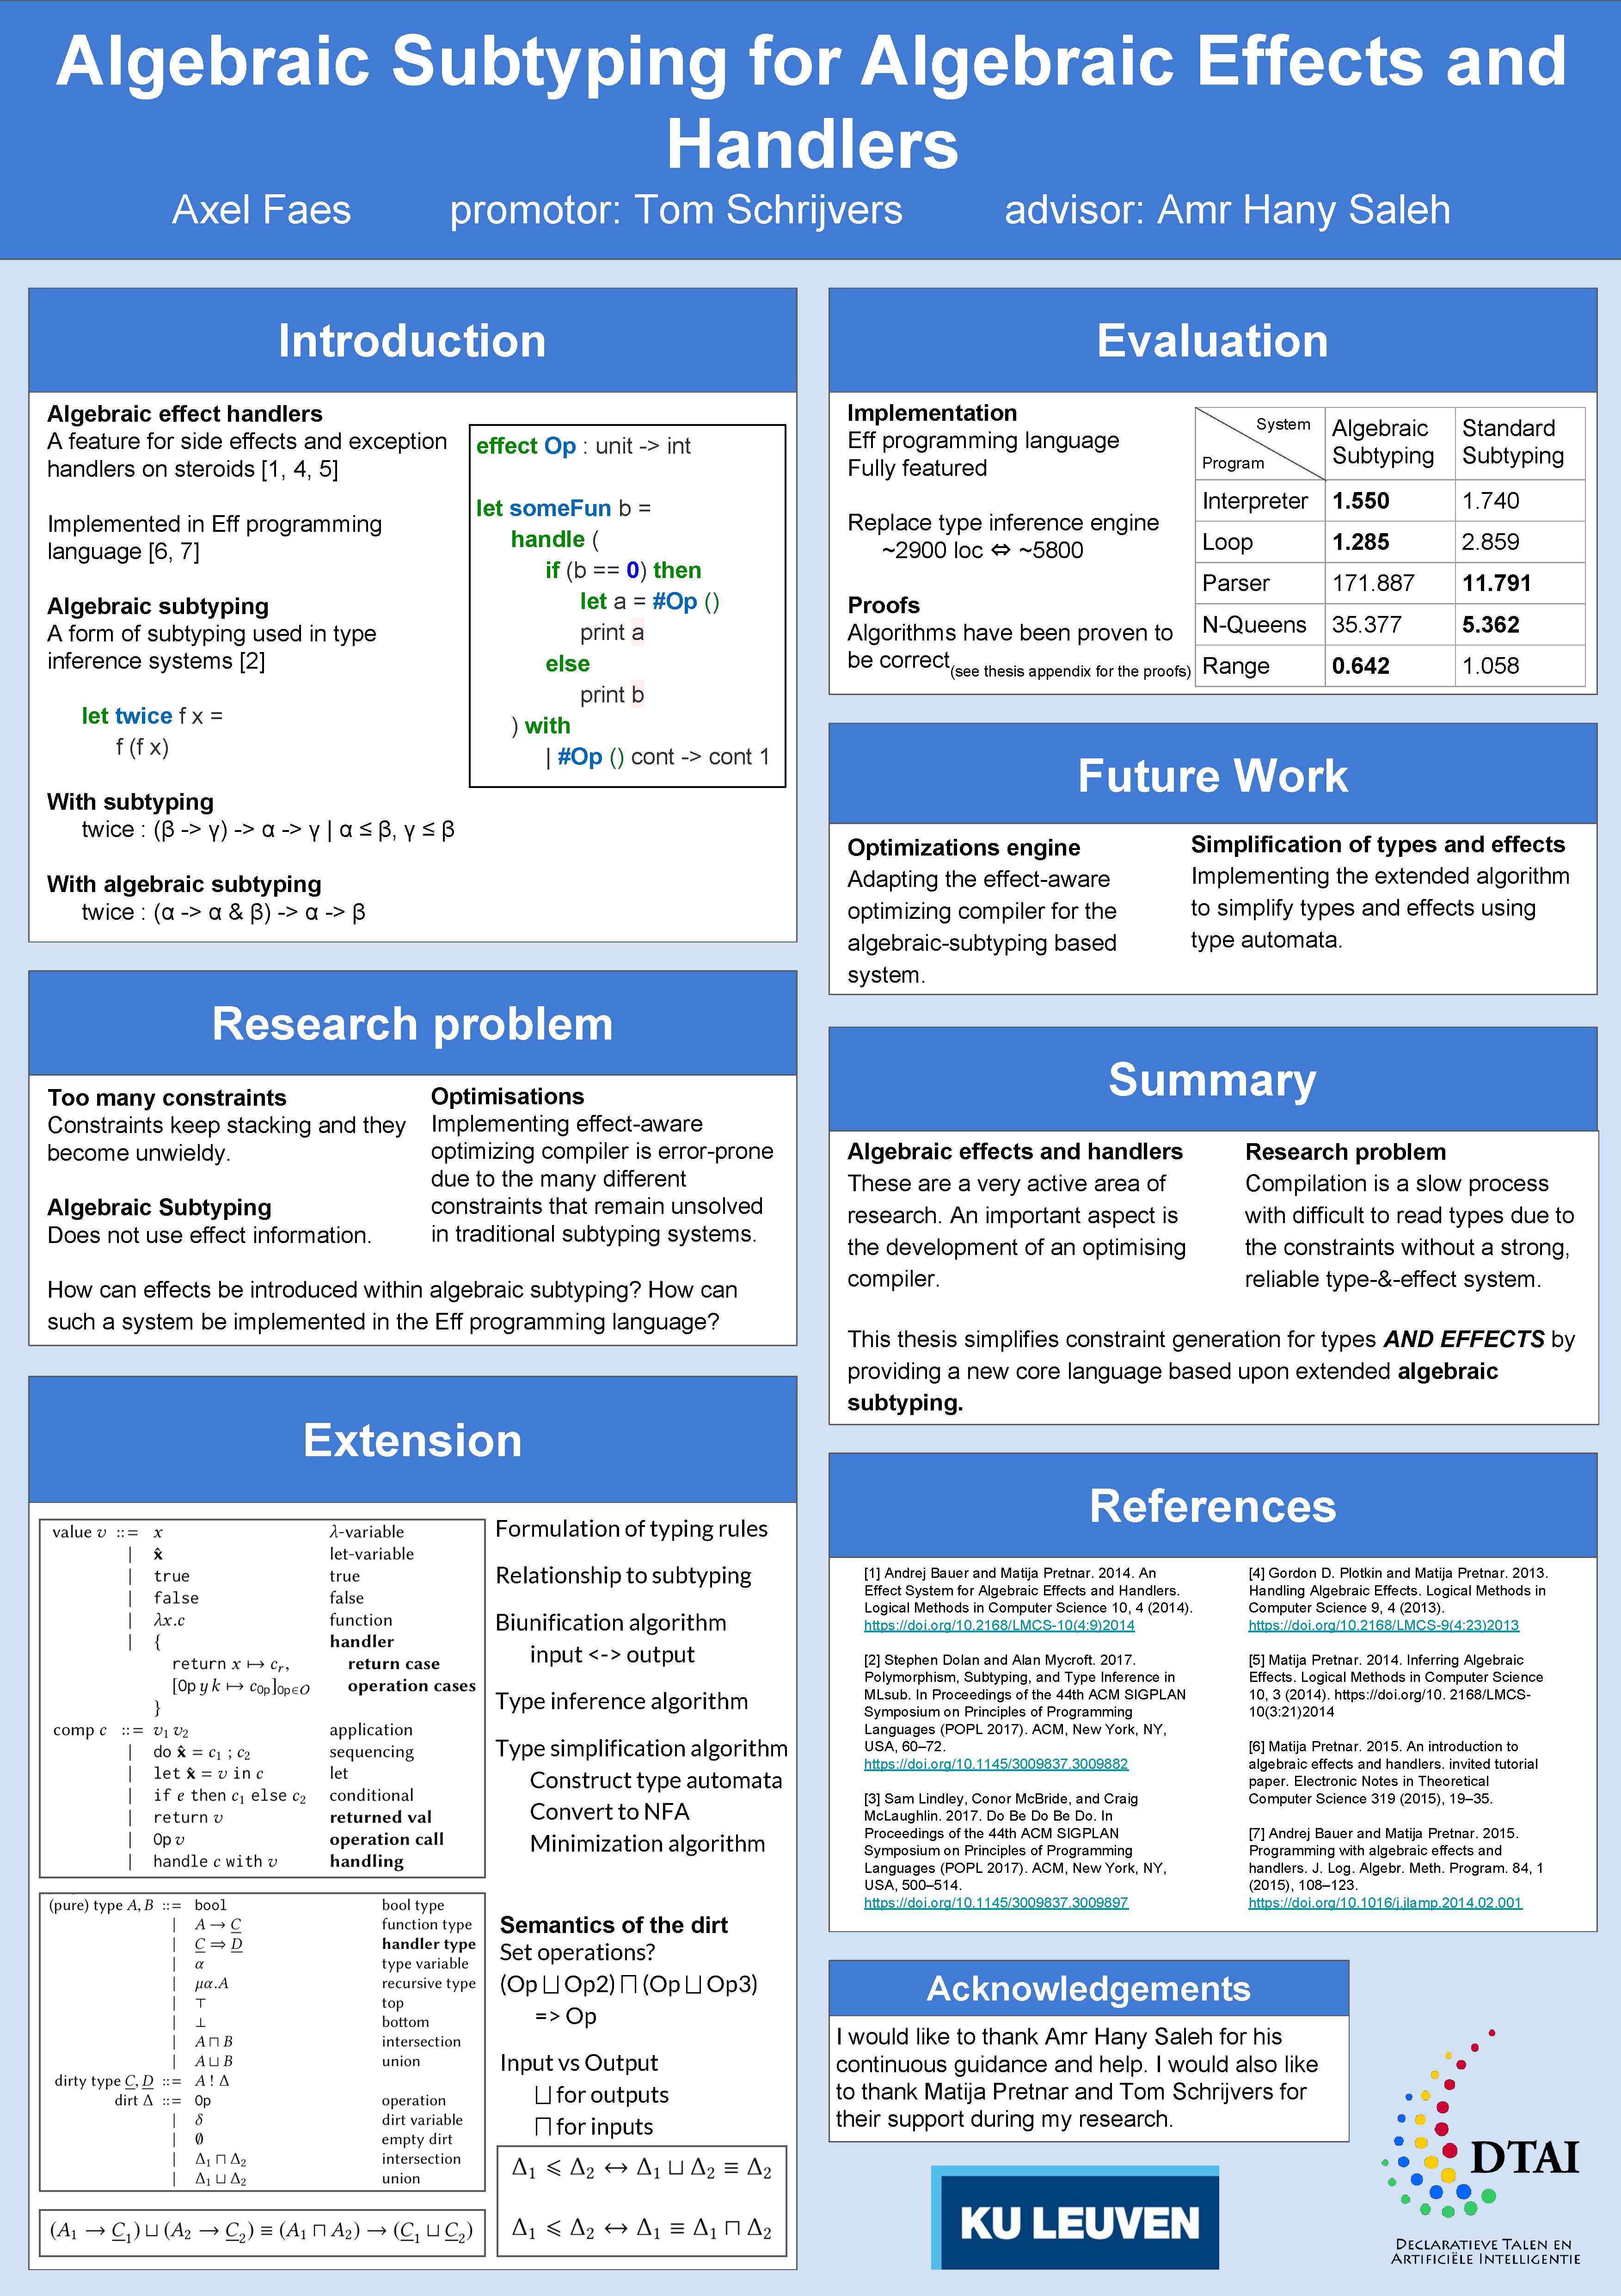
\includepdf[]{../poster/poster.pdf}

%% Acknowledgments
\begin{acks}
  I would like to thank Amr Hany Saleh for his continuous guidance and help.
\end{acks}

\bibliography{bib/main}
\nocite{*}

\end{document}
